\exercisesection{3}

\begin{enumerate}
\def\labelenumi{\arabic{enumi}.}
\tightlist
\item
  \begin{enumerate}
  \def\labelenumii{(\alph{enumii})}
  \tightlist
  \item
    设 A 是一个环（不必交换），\(I_{s}\) （相应地 \(I_{d}\) ）是 A 中没有左逆（相应地右逆）的元素组成的集合。证明下列条件等价：(1) \(I_{s}\) 中两个元素之和属于 \(I_{s}\) ；(2) \(I_{s}\) 是一个左理想；(3) 在由 \(\neq A\) 的诸左理想组成的集合中存在一个最大的左理想 J。若这些条件成立，则反环 \(A^{0}\) 也满足这些条件，\(I_{s} = I_{d} = J\) ，J 是 A 的唯一的极大（左或右）理想，因而是 A 的 Jacobson 根，每个元素 \(x \notin J\) 都可逆，且 A/J 是一个域（参看《代数》第 VIII 章 §6 第 3 节）。这时我们也说 A 是一个局部环。
  \end{enumerate}
\end{enumerate}

\begin{enumerate}
\def\labelenumi{(\alph{enumi})}
\setcounter{enumi}{1}
\tightlist
\item
  证明：在局部环中，除 0 与 1 外不存在其他幂等元。
\end{enumerate}

\begin{enumerate}
\def\labelenumi{\arabic{enumi}.}
\setcounter{enumi}{1}
\tightlist
\item
  \begin{enumerate}
  \def\labelenumii{(\alph{enumii})}
  \tightlist
  \item
    设 A 是一个（交换）局部环，其极大理想 m 是主理想，且满足 \(\bigcap_{n\geqslant1}m^{n}=0\) （参看第 III 章 §3 第 2 节命题 4 的推论）。证明 A 的既 \(\neq0\) 又 \(\neq A\) 的理想只有诸幂 \(m^{n}\) ；由此推出 A 是 Noether 环，并且*或者是一个离散赋值环（第 VI 章）*，或者是一个使 1 为不可分解幂等元的拟主理想环（《代数》第 VII 章 §1 习题 6）。
  \end{enumerate}
\end{enumerate}

\begin{enumerate}
\def\labelenumi{(\alph{enumi})}
\setcounter{enumi}{1}
\tightlist
\item
  设 A 是由在 0 的一个邻域中定义且连续、并在点 0 可微的实值函数在点 t = 0 处的芽组成的环（《一般拓扑学》第 I 章第 3 版 § 6 第 10 节）。证明 A 是一个局部环，其极大理想 m 由函数 \(j: t \mapsto t; m^{n} \neq 0\) （对所有 n）的芽生成，但 A 不是主理想整环。若 c 是函数 \(t \mapsto \exp(-1/t^{2})\) 的芽，p 是 A 的一个不含 c 的素理想，证明商环 B = A/p 是一个局部整环，它不是主理想整环，而其极大理想是主理想。
\end{enumerate}

¶ 3. 设 A 是一个局部环（不必交换，参看习题 1），m 是它的 Jacobson 根。

\begin{enumerate}
\def\labelenumi{(\alph{enumi})}
\item
  设 L 是一个自由左 A-模，\(x \neq 0\) 是 L 的一个元素。设 \((e_{\iota})_{\iota \in I}\) 是 L 的一个基，对于它，x 的 \(\neq 0\) 分量的个数尽可能地小；若 \(x = \sum_{\iota \in I} \xi_{\iota} e_{\iota}\) ，设 J 是 \(\iota \in I\) 中使 \(\xi_{\iota} \neq 0\) 的元素组成的集合。证明：诸 \(\xi_{\iota} (\iota \in J)\) 中任何一个都不属于 A 中由其余分量生成的右理想。
\item
  在 (a) 的假设与记号下，设 P、Q 是 L 的两个互补子模，且 \(x \in P\) ；对每个 \(\iota \in I\) ，写 \(e_{\iota} = y_{\iota} + z_{\iota}\) ，其中 \(y_{\iota} \in P\) ，\(z_{\iota} \in Q\) 。证明：诸 \(y_{\iota}\) （其中 \(\iota \in J\) ）与诸 \(e_{\iota}\) （其中 \(\iota \notin J\) ）构成的族是 L 的一个基。（利用 (a) 证明：若 \(z_{\kappa} = \sum_{\iota \in I} \zeta_{\kappa_{\iota}} e_{\iota}\) ，则分量 \(\zeta_{\kappa_{\iota}}\) （其中 \(\kappa \in J\) 且 \(\iota \in J\) ）必属于 m，并利用命题 4 的推论 2。）由此推出：存在 P 的一个自由子模，它包含 x 且是 P 的直因子。
\item
  证明每个投射 A-模 P 都是自由的（利用 Kaplansky 定理（《代数》第 II 章 § 2 习题 4），归结到 P 由可数多个元素生成的情形，并对该情形应用 (b)）。
\item
  给出一个局部环 A 和一个平坦 A-模 M 的例子，使 M 不是自由的且满足 mM = M（取 \(A = \mathbf{Z}_{(p)}\) ）。*（在第 III 章 § 3 中，我们将给出 Noether 局部环 A 上的非自由忠实平坦 A-模的例子。）*
\item
  设 A 是一个局部环，M 是一个有限生成平坦 A-模。证明 M 是自由 A-模（利用第 I 章 § 2 习题 23 (e)）。
\end{enumerate}

\begin{enumerate}
\def\labelenumi{\arabic{enumi}.}
\setcounter{enumi}{3}
\item
  设 A 是一个局部环（不必交换），m 是它的 Jacobson 根。设 M、N 是两个自由 A-模（不一定有限生成），\(u: M \rightarrow N\) 是一个同态，使得 \(1 \otimes u: M/mM \rightarrow N/mN\) 是双射。证明 u 是双射。（先证明 u 是满射，再证明 u 是单射，归结到 M 与 N 都是有限生成的情形，并分别利用命题 4 的推论 1 与命题 6。）
\item
  用例子说明：命题 7 不能推广到局部环 A 不是约化环的情形。
\item
  \begin{enumerate}
  \def\labelenumii{(\alph{enumii})}
  \tightlist
  \item
    设 M 是《代数》第 VII 章 §3 习题 22 (h) 中定义的 Z-模；设 T 是 M 的扭子模。证明：对每个素数 p，\(\mathrm{T}_{(p)}\) 作为 \(\mathrm{M}_{(p)}\) 的子模是 \(\mathrm{M}_{(p)}\) 的直因子，尽管 T 不是 M 的直因子。
  \end{enumerate}
\end{enumerate}

\begin{enumerate}
\def\labelenumi{(\alph{enumi})}
\setcounter{enumi}{1}
\tightlist
\item
  设 \(\mathbf{M}\) 是《代数》第 VII 章 § 3 习题 5 中定义的 \(\mathbf{Z}\) -模；证明：对每个素数 \(p\) ，\(\mathrm{M}_{(p)}\) 是自由 \(\mathbf{Z}_{(p)}\) -模，尽管 \(\mathbf{M}\) 不是自由 \(\mathbf{Z}\) -模。
\end{enumerate}

\begin{enumerate}
\def\labelenumi{\arabic{enumi}.}
\setcounter{enumi}{6}
\item
  设 A 是一个环，\((\mathrm{S}_{\lambda})_{\lambda \in L}\) 是 A 的乘性子集的一个族，使得对 A 的每个极大理想 m，存在 \(\lambda \in L\) 满足 \(m \cap S_{\lambda} = \varnothing\) （参看 §2 习题 8）。设 M、N 是两个 A-模，u: M → N 是一个同态。为使 u 是满射（相应地，单射、双射、零同态），必须且只需：对所有 \(\lambda \in L\) ，\(S_{\lambda}^{-1}u\) : \(S_{\lambda}^{-1}M \to S_{\lambda}^{-1}N\) 是满射（相应地，单射、双射、零同态）。第 3 节定理 1 的诸推论可以怎样推广？
\item
  设 A 是一个环，B 是一个 A-代数（不必交换），E 是一个有限生成左 B-模。
\end{enumerate}

\begin{enumerate}
\def\labelenumi{(\alph{enumi})}
\item
  设 S 是 A 的一个乘性子集，并给 \(S^{-1}B = S^{-1}A \otimes_{A} B\) 赋以它的 \(S^{-1}A\) -代数结构；于是可以把 \(S^{-1}E\) 视为一个左 \(S^{-1}B\) -模（《代数》第 VIII 章 § 7 第 1 节），它同构于 \(S^{-1}B \otimes_{B} E\) 。证明：若 E 是平坦 B-模，则 \(S^{-1}E\) 是平坦 \(S^{-1}B\) -模。
\item
  设 \((\mathbf{S}_{\lambda})_{\lambda \in L}\) 是 A 的乘性子集的一个族，使得对 A 的每个极大理想 m，存在 \(\lambda \in L\) 满足 \(m \cap S_{\lambda} = \varnothing\) 。证明 \(\bigoplus_{\lambda \in L} S_{\lambda}^{-1} B\) 是一个忠实平坦 B-模（左模或右模；参看 § 2 习题 8）。证明：若对所有 \(\lambda \in L\) ，\(S_{\lambda}^{-1} E\) 是平坦（相应地，忠实平坦）\(S_{\lambda}^{-1} B\) -模，则 E 是平坦（相应地，忠实平坦）B-模（利用第 I 章 § 3 习题 9，取 \(C_{\lambda} = S_{\lambda}^{-1} A\) ）。
\item
  假设诸 \(S_{\lambda}\) 满足条件 (b)，且 L 有限。证明：若对每个 \(\lambda \in L\) ，\(S_{\lambda}^{-1}E\) 是有限生成投射 \(S_{\lambda}^{-1}B\) -模，则 E 是有限生成投射 B-模。
\end{enumerate}

\begin{enumerate}
\def\labelenumi{\arabic{enumi}.}
\setcounter{enumi}{8}
\item
  证明：为使一个（交换）环 A 是绝对平坦的（第 I 章 § 2 习题 17），必须且只需对 A 的每个极大理想 m，\(A_{m}\) 都是域（注意绝对平坦局部环必为域，并利用命题 15 的推论）。
\item
  设 A、B 是两个环，\(\rho: A \rightarrow B\) 是一个同态，q 是 B 的一个素理想，\(p = \bar{\rho}^{-1}(q)\) 。假设存在一个 B-模 N，使得 \(N_{q}\) 是一个不化为 0 的平坦 A-模，且 \(N_{q}\) 是一个有限生成 \(A_{p}\) -模；则素理想 p 在 A 中是极小的。（注意 \(N_{p}\) 这时是一个忠实平坦 \(A_{p}\) -模，并利用 §2 第 5 节命题 11 的推论 4。）
\item
  设 A 是一个环，a 是 A 的一个理想，S 是由其在 A/a 中的典范像不是零因子的那些元素组成的 A 的乘性子集；设 \(\Phi\) 是 A 的与 S 不相交的理想组成的集合中的极大元组成的集合（因而诸理想 \(p \in \Phi\) 是素的，参看 §2 第 5 节命题 11）。证明：a 关于诸理想 \(p \in \Phi\) 的饱和的交就是 a 本身（归结到 a = 0 的情形，并利用定理 1 的推论 1）。
\end{enumerate}

¶ 12. 设 \(A = \prod_{i=1}^{n} A_i\) 是有限多个局部环 \(A_i\) 组成的族的乘积，这些局部环典范地等同于 \(A\) 的理想。设 \(B\) 是 \(A\) 的一个子环，使得 \(\text{pr}_i B = A_i\) 对 \(1 \leqslant i \leqslant n\) 成立。证明 \(B\) 是至多 \(n\) 个局部环的直复合，并且是 \(n\) 个局部环的直复合仅当 \(B = A\) 时才可能。（对 \(n\) 作归纳，考虑由 \(a_i = B \cap A_i\) 给出的 \(B\) 的理想。相继考察 \(a_i = A_i\) 至少对一个指标 \(i\) 成立的情形，以及 \(a_i \neq A_i\) 对所有 \(i\) 成立的情形。注意：若 \(a_i \neq A_i\) ，则 \(B\) 的每个极大理想都包含 \(a_i\) ，并且通过考虑环 \(B / a_i\) ，断言至多存在 \(n - 1\) 个属于 \(B\) 的互不相同的极大理想；若这时 \(B\) 不是局部环，则利用归纳假设与习题 1 (b) 归结到 \(a_j = A_j\) 对某个 \(j \neq i\) 成立的情形。）给出一个例子，其中 \(n > 1\) 且 \(B\) 是局部环，但不与任何 \(A_t\) 同构（取诸 \(A_t\) 为同一域 \(K\) 上的代数，其极大理想 \(m_t\) 的平方为零）。

¶ 13. 设 G 是一个有限群，其阶 n 是一个素数 p 的幂 \(p^{f}\) ，而 K 是特征为 p 的域。

\begin{enumerate}
\def\labelenumi{(\alph{enumi})}
\item
  设 E 是一个 G 在其上作用的有限集（《代数》第 I 章 § 7 第 2 节）；若 \(E'\) 是 E 中对所有 \(g \in G\) 都不变的元素组成的集合，证明 \(\text{Card}(E) \equiv \text{Card}(E') \pmod{p}\) 。由此推出：若 G 不化为它的单位元 e，则 G 的中心 Z 不化为 e（让 G 通过内自同构作用在它自身上）。断言 G 是可解的（《代数》第 I 章 § 6 习题 14）。
\item
  设 V 是 K 上的一个向量空间，\(\rho\) 是 G 到 \(\mathbf{GL}(V)\) 的一个同态。设 \(V'\) 是 \(x \in V\) 中在线性映射 \(\rho(g)\) （其中 \(g \in G\) ）下不变的元素组成的集合。证明：若 \(V'\) 化为 0，则 V 必化为 0。（若 \(x \in V\) 且 \(x \neq 0\) ，对由诸元素 \(\rho(g).x\) （其中 \(g \in G\) ）生成的 V 的加法子群 E 应用 (a)。）
\item
  设 \(\mathbf{A} = \mathbf{K}^{(\mathbf{G})}\) 是群 \(\mathbf{G}\) 在 \(\mathbf{K}\) 上的代数（《代数》第 III 章 § 1），\(\mathbf{I}\) 是 \(\mathbf{A}\) 的（ \(\mathbf{K}\) 上的）由诸元素 \(1 - g\) （其中 \(g \in \mathbf{G}\) ）生成的向量子空间。证明 \(\mathbf{I}\) 是 \(\mathbf{A}\) 的 Jacobson 根，且 \(\mathbf{A} / \mathbf{I}\) 同构于 \(\mathbf{K}\) （利用 (b) 及 Jacobson 根的定义）；由此推出 \(\mathbf{I}\) 是幂零的。
\item
  设 V 是一个有限生成 A-模，V′ 是 V 中对所有 \(g \in G\) 满足 g.x = x 的元素 x 组成的集合。证明下列不等式成立
\end{enumerate}

\[
(*) \dim_ {\mathbb {K}} (\mathrm{V}) \leqslant n. \dim_ {\mathbb {K}} (\mathrm{V} / \mathrm{IV}); \quad (* *) \dim_ {\mathbb {K}} (\mathrm{V}) \leqslant n. \dim_ {\mathbb {K}} (\mathrm{V} ^ {\prime}).
\]

（为建立 (*)，利用命题 4 的推论 2；通过考虑 V 在 K 上的对偶向量空间推出 (**)。）为使不等式 (*) （相应地 (**)）两边相等，必须且只需 V 是自由 A-模（参看命题 5 的推论 1）。

\begin{enumerate}
\def\labelenumi{\arabic{enumi}.}
\setcounter{enumi}{13}
\tightlist
\item
  设 A 是一个环，它不必交换，且其 Jacobson 根 m 使得 A/m 是一个域；设 M 是一个有限生成自由 A-模。
\end{enumerate}

\begin{enumerate}
\def\labelenumi{(\alph{enumi})}
\item
  设 \(\mathbf{M}'\) 是另一个有限生成自由 A-模，\(u: \mathbf{M} \to \mathbf{M}'\) 是一个同态，使得 \(u(\mathbf{M})\) 是 \(\mathbf{M}'\) 的一个直因子；数 \(\dim(\mathbf{M})\) 称为 \(u\) 的秩，记作 \(\operatorname{rg}(u)\) 。对这样的同态，\(\operatorname{Ker}(u)\) 是 \(\mathbf{M}\) 的直因子，且 \(\operatorname{rg}(u) = \dim(\mathbf{M}) - \dim(\operatorname{Ker}(u))\) ；为使 \(u\) 是单射（相应地满射），必须且只需 \(\operatorname{rg}(u) = \dim(\mathbf{M})\) （相应地 \(\operatorname{rg}(u) = \dim(\mathbf{M}')\) ）。转置 \(^t u\) 使得 \(^t u(\mathbf{M}'*)\) 是 \(\mathbf{M}^*\) 的直因子，且 \(\operatorname{rg}(^t u) = \operatorname{rg}(u)\) 。
\item
  设 \(n = \dim(\mathbf{M})\) 。\(\mathbf{M}\) 的维数为 1（相应地 \(n - 1\) ）的直因子称为直线（相应地超平面）。一个异于恒等映射的自同构 \(u \in \mathbf{GL}(\mathbf{M})\) 称为一个平延，如果存在超平面 \(\mathbf{H}\) 含于 \(\mathbf{M}\) ，它的所有元素在 \(u\) 下不变；这时 \(u(x) = x + a\phi(x)\) ，其中 \(\phi\) 是 \(\mathbf{M}\) 上的一个线性形式，使得 \(\mathbf{H} = \operatorname{Ker}(\phi)\) ，而 \(a \in \mathbf{H}\) ；证明其逆。若 \(\mathbf{A}\) 交换，证明每个行列式为 1 的自同构 \(u \in \mathbf{GL}(\mathbf{M})\) 都是平延之积（注意，在 \(u\) 关于 \(\mathbf{M}\) 的任意一组基的矩阵中，每一列至少含有 \(\mathbf{A}\) 的一个可逆元素，且形如 \(I + E_{ij} (i \neq j)\) 的矩阵是一个平延的矩阵）。
\item
  给出一个自同构 \(u \in \mathbf{GL}(\mathbf{M})\) 的例子，使 \(1 - u\) 的核不是 \(\mathbf{M}\) 的直因子（取 \(\mathbf{A}\) 为局部环 \(\mathbf{K}[[\mathbf{X}]]\) ，即域 \(\mathbf{K}\) 上一个未定元的形式幂级数环，并取 \(\mathbf{M} = \mathbf{A}\) ）。
\item
  给出 M 的直因子 N、P（必然是自由的）的例子，使得 \(N + P\) 与 \(N \cap P\) 都不是 M 的直因子。（取 A = K{[}X{]}/(X²)，其中 K 是一个域，M = A²。）
\end{enumerate}

¶ 15. 设 A 是一个（交换）环，M 是一个 A-模。

\begin{enumerate}
\def\labelenumi{(\alph{enumi})}
\item
  为使 M 的子模 \(M'\) 是纯的（第 I 章 §2 习题 24），必须且只需对 A 的每个极大理想 m，\(M_{m}'\) 都是 \(A_{m}\) -模 \(M_{m}\) 的纯子模（利用第 3 节定理 1）。
\item
  假设 A 是以 m 为极大理想的局部环，M 是一个有限生成自由 A-模。为使 M 的一个有限生成子模 \(M'\) 是纯的，必须且只需它是 M 的直因子。（利用第 2 节命题 5 的推论 1，归结为证明：若 \(M' \subset mM\) ，则 \(M'\) 仅当 \(M' = 0\) 时才可能是 M 的纯子模。）
\end{enumerate}

\begin{enumerate}
\def\labelenumi{\arabic{enumi}.}
\setcounter{enumi}{15}
\tightlist
\item
  设 \((\mathbf{A}_{\lambda}, f_{\mu \lambda})\) 是局部环的一个正向系，使得诸 \(f_{\mu \lambda}\) 都是局部同态；设 \(m_{\lambda}\) 是 \(\mathbf{A}_{\lambda}\) 的极大理想，\(\mathbf{K}_{\lambda} = \mathbf{A}_{\lambda} / m_{\lambda}\) 。则 \(\mathbf{A} = \varinjlim \mathbf{A}_{\lambda}\) 是一个局部环，其极大理想为 \(m = \varinjlim m_{\lambda}\) ，剩余域为 \(\mathbf{K} = \varinjlim \mathbf{K}_{\lambda}\) 。此外，若 \(m_{\mu} = \mathbf{A}_{\mu} m_{\lambda}\) 对 \(\lambda < \mu\) 成立，则 \(m = Am_{\lambda}\) 对所有 \(\lambda\) 成立。
\end{enumerate}

\exercisesection{4}

\begin{enumerate}
\def\labelenumi{\arabic{enumi}.}
\item
  设 \((\mathbf{X}_{\alpha}, f_{\alpha\beta})\) 是拓扑空间的一个逆向系，其指标集是有向的，\(X = \varprojlim X_{\alpha}\) ，而 \(f_{\alpha}\) 是 X 到 \(X_{\alpha}\) 的典范映射。假设对所有 \(\alpha, f_{\alpha}\) 都是满射；证明：若诸 \(X_{\alpha}\) 都不可约，则 X 不可约（参看《一般拓扑学》第 I 章 §4 第 4 节命题 9 的推论）。特别地，不可约空间的任意乘积都不可约。
\item
  不可约空间中的一点 \(x\) 称为该空间 \(\mathbf{X}\) 的泛点，如果 \(\{x\}\) 在 \(\mathbf{X}\) 中处处稠密。
\end{enumerate}

\begin{enumerate}
\def\labelenumi{(\alph{enumi})}
\tightlist
\item
  若 \(\mathbf{X}\) 是一个 Kolmogoroff 空间（《一般拓扑学》第 I 章 § 1 习题 2），它至少有一个泛点；若 \(\mathbf{X}\) 是一个可达空间（《一般拓扑学
\end{enumerate}

》第 I 章 § 8 习题 1），则除非它仅由一点组成，它不可能有泛点。

\begin{enumerate}
\def\labelenumi{(\alph{enumi})}
\setcounter{enumi}{1}
\item
  给出一个无限的不可约可达空间的例子（参看《一般拓扑学》第 I 章 § 8 习题 5）。
\item
  设 X、Y 是两个都有泛点的不可约空间；再假设 Y 只有唯一的泛点 y。设 \(f: X \to Y\) 是一个连续映射；为使 \(f(X)\) 在 Y 中稠密，必须且只需对 X 的每个泛点 x 都有 \(f(x) = y\) 。
\item
  设 \((\mathbf{X}_{\alpha}, f_{\alpha \beta})\) 是不可约空间的一个逆向系，其指标集是有向的；假设每个 \(\mathbf{X}_{\alpha}\) 都有唯一的泛点 \(x_{\alpha}\) 。证明：若对 \(\alpha \leqslant \beta, f_{\alpha \beta}(\mathbf{X}_{\beta})\) 在 \(\mathbf{X}_{\alpha}\) 中稠密，则 \(\mathbf{X} = \varprojlim \mathbf{X}_{\alpha}\) 不可约且只有唯一的泛点（方法同习题 1）。
\end{enumerate}

\begin{enumerate}
\def\labelenumi{\arabic{enumi}.}
\setcounter{enumi}{2}
\item
  设 X 是一个拓扑空间，\((Y_{\alpha})\) 是 X 的子空间的一个右有向族；证明：若每个子空间 \(Y_{\alpha}\) 都不可约，且 X 是族 \((Y_{\alpha})\) 之并，则 X 不可约。由此给出一个例子：X 是 Kolmogoroff 空间，每个 \(Y_{\alpha}\) 都有泛点，但 X 没有泛点。
\item
  设 Y 是只有唯一泛点 y 的不可约空间，X 是一个拓扑空间，\(f: X \rightarrow Y\) 是一个连续映射。
\end{enumerate}

\begin{enumerate}
\def\labelenumi{(\alph{enumi})}
\item
  设 \(\mathbf{Z}\) 是 \(\mathbf{X}\) 的一个不可约分支，它与 \(f^{-1}(y), f(\mathbf{Z})\) 中的前者相交；则其像在 \(\mathbf{Y}\) 中稠密。
\item
  给出一个例子，其中 \(f(\mathbf{X})\) 在 \(\mathbf{Y}\) 中稠密，但 \(f^{-1}(y)\) 为空（取 \(\mathbf{X}\) 为 \(\mathbf{Y}\) 的一个子空间）。
\item
  证明：若 \(\mathbf{Z}\) 有一个泛点 \(z\) 且 \(f(\mathbf{Z})\) 在 \(\mathbf{Y}\) 中稠密，则 \(f(z) = y\) ，且 \(z\) 是 \(\mathbf{Z} \cap f^{-1}(y)\) 的一个泛点。
\end{enumerate}

\begin{enumerate}
\def\labelenumi{\arabic{enumi}.}
\setcounter{enumi}{4}
\item
  设 G 是一个连通的半拓扑群（《一般拓扑学》第 III 章 § 1 习题 2）。证明：若 G 只有有限多个不可约分支，则它必然不可约（注意诸不可约分支都可由包含单位元 e 的那个不可约分支经左平移或右平移得到）。
\item
  设 \(\mathbf{X}\) 是一个拓扑空间。
\end{enumerate}

\begin{enumerate}
\def\labelenumi{(\alph{enumi})}
\item
  设 x 是 X 的一点，U 是 x 的一个只有有限多个不可约分支的开邻域。证明存在 x 的一个邻域 V，使得包含于 V 的每个邻域都是连通的。
\item
  假设 X 的每一点都有一个只含有限多个不可约分支的开邻域。证明下列性质等价：
\end{enumerate}

(α) X 的诸不可约分支都是开的。

(β) X 的诸不可约分支与它的诸连通分支相同。

(γ) X 的诸连通分支都不可约。

(δ) X 的两个互不相同的不可约分支不相交。

\begin{enumerate}
\def\labelenumi{\arabic{enumi}.}
\setcounter{enumi}{6}
\item
  设 X 是一个紧可度量化空间，R 是 X 上的一个开等价关系，使得商空间 X/R 不可约。证明存在一点 \(x \in X\) ，它模 R 的类处处稠密。（首先注意 X 的每个关于 R 饱和的开子集都处处稠密。然后利用 Baire 定理。）
\item
  证明两个 Noether 空间的乘积是 Noether 空间。（若 X 与 Y 是 Noether 空间，A 是 \(X \times Y\) 的一个开子集，证明：对所有 \(x \in pr_{1}A\) ，存在 x 的一个开邻域 V，使得 \(V \times A(x) \subset A\) ，并由此推出 A 是拟紧的。）
\item
  \begin{enumerate}
  \def\labelenumii{(\alph{enumii})}
  \tightlist
  \item
    证明交换环的素谱是一个 Kolmogoroff 空间（《一般拓扑学》第 I 章 § 1 习题 2），其中每个不可约分支都有（唯一的）泛点。
  \end{enumerate}
\end{enumerate}

\begin{enumerate}
\def\labelenumi{(\alph{enumi})}
\setcounter{enumi}{1}
\tightlist
\item
  设 A 是一个整环，\(\xi = (0)\) 是 \(\mathbf{X} = \operatorname{Spec}(\mathbf{A})\) 的泛点。为使点 \(\xi\) 在 X 中孤立，必须且只需 A 的诸 \(\neq 0\) 素理想的交是一个 \(\neq 0\) 的理想。给出一个具有此性质的局部环的例子。
\end{enumerate}

\begin{enumerate}
\def\labelenumi{\arabic{enumi}.}
\setcounter{enumi}{9}
\item
  设 A 是一个环，N 是它的幂零根。为使 A 的谱是离散的，必须且只需 A/N 是有限多个域的直复合。
\item
  设 K 是一个域，A 是多项式环 K{[}X, Y{]}，B 是商环 A/(XY)；证明 Spec(B) 是连通的，但有两个互不相同的不可约分支。
\item
  设 Y 是一个完全正则空间，\(\mathbf{A} = \mathcal{C}^{\infty}(\mathbf{Y}; \mathbf{R})\) ，\(\mathbf{B} = \mathcal{C}(\mathbf{Y}; \mathbf{R})\) 。证明 Y 的 Stone-Čech 紧化 \(\beta Y\) 典范地等同于 \(\operatorname{Spec}(A)\) 的一个处处稠密子空间，并且典范地等同于 \(\operatorname{Spec}(B)\) 的一个处处稠密子空间。
\item
  设 \(\mathbf{A}\) 是一个环，\(\mathbf{X} = \operatorname{Spec}(\mathbf{A})\) 是它的谱。
\end{enumerate}

\begin{enumerate}
\def\labelenumi{(\alph{enumi})}
\item
  若 X 的一个子集 F 是闭的，它就具有下列两个性质：(α) 对所有 p ∈ F，有 V(p) ⊂ F；(β) 对所有 p ∉ F，存在 V(p) 的一个闭子集，它包含 F ∩ V(p) 但不包含 p。
\item
  假设 X 是 Noether 的。证明 X 的每个具有 (a) 中性质 \((\alpha)\) 与 \((\beta)\) 的子集 F 在 X 中是闭的（考虑 \(\overline{F}\) 的不可约分支，并利用习题 9 (a)）。
\item
  沿用习题 12 的记号，取 Y 为 R 的区间 {[}0, 1{]}。证明 Y 在 X = Spec(A) 中不是闭的（参看 § 2 习题 15），但满足 (a) 的条件 ( \(\alpha\) ) 与 ( \(\beta\) )。
\end{enumerate}

\begin{enumerate}
\def\labelenumi{\arabic{enumi}.}
\setcounter{enumi}{13}
\tightlist
\item
  设 A 是一个环，\(\mathbf{X} = \operatorname{Spec}(\mathbf{A})\) 是它的谱，P 是 A 的极小素理想组成的集合。
\end{enumerate}

\begin{enumerate}
\def\labelenumi{(\alph{enumi})}
\item
  设 \(R_{\mathfrak{p},\mathfrak{p}^{\prime}}\) 是对称且自反的关系：“存在 A 的一个素理想 \(\mathfrak{p}''\) ，它包含 \(\mathfrak{p} + \mathfrak{p}'''\) ，并且位于 P 的元素 \(\mathfrak{p},\mathfrak{p}'\) 之间”；设 S 是这样的等价关系：它的图是包含 R 的图的诸等价关系的图中最小的一个（《集合论》第 II 章 § 6 习题 10）。证明：若 I 是关于 S 的一个等价类，则集合 \(V_{I} = \bigcup_{\mathfrak{p}\in I}V(\mathfrak{p})\) 是连通的。
\item
  证明：若 P 是有限的（特别地，若 A 是 Noether 的），则诸 \(V_{I}\) 是 X 的连通分支。这一结果能否推广到 P 无限的情形（参看习题 12）？
\end{enumerate}

¶ 15. 设 A 是一个环，a 是 A 的一个有限生成理想。证明下列性质等价：(α) \(a^{2} = a\) ；(β) A 由一个幂等元生成；(γ) V(a) 在 X = Spec(A) 中既开又闭，且 a 在满足 r(b) = r(a) 的诸理想 b 中是最小的（利用 § 2 命题 4 的推论 3）。给出一个例子，其中 \(a^{2} = a\) ，a 不是有限生成的，且不含幂等元（参看 § 2 习题 15）。

¶ 16. (a) 设 A 是一个绝对平坦的（交换）环（第 I 章 §2 习题 17）。证明 X = Spec(A) 是一个全不连通的紧空间，A 的每个素理想 p 都是极大的，并且 \(A_{p}\) 典范地同构于域 A/p（首先证明：对所有 f ∈ A，V(f) 在 X 中既开又闭；另一方面利用 §3 习题 9）。

\begin{enumerate}
\def\labelenumi{(\alph{enumi})}
\setcounter{enumi}{1}
\tightlist
\item
  证明映射 \(\mathfrak{a}\mapsto\mathrm{V}(\mathfrak{a})\) 是 A 的理想组成的集合到 X 的闭子集组成的集合上的一个双射。此外，下列条件等价：( \(\alpha\) ) V(a) 是开的；( \(\beta\) ) a 是有限生成的；( \(\gamma\) ) a 由一个幂等元生成；( \(\delta\) ) A/a 是一个投射 A-模。
\end{enumerate}

* (c) 设 \(\tilde{A}\) 是 \(X\) 上的结构环层。证明每个 \(\tilde{A}\) -模 \(\mathcal{F}\) 都形如 \(\tilde{E}\) ，其中 \(E\) 是一个在相差一个唯一同构的意义下确定的 A-模（取 \(E = \Gamma(X, \mathcal{F})\) ，并利用 \(X\) 的每一点都有一个由既开又闭的邻域组成的基本系这一事实）。设 \(a\) 是 \(A\) 的任意一个理想，证明 \(\operatorname{Hom}_A(a, E)\) 等同于 \(\Gamma(X - V(a), \tilde{E})\) （注意 \(X - V(a)\) 是诸 \(X_e\) 之并，其中 \(e\) 取遍幂等元 \(e \in a\) 组成的集合）。由此推出：为使 \(E\) 是一个内射 A-模，必须且只需 \(\tilde{E}\) 是松弛的。*

\begin{enumerate}
\def\labelenumi{(\alph{enumi})}
\setcounter{enumi}{3}
\tightlist
\item
  设 A 是一个环，\(\mathfrak{N}\) 是它的幂零根。下列性质等价：
\end{enumerate}

(α) \(A/\mathfrak{N}\) 是绝对平坦的。

(β) \(\mathbf{X} = \operatorname{Spec}(\mathbf{A})\) 是 Hausdorff 的。

(γ) X 的每一点都是闭的（换言之，A 的每个素理想都是极大的）。

（利用 § 3 的习题 9。）

¶ 17. * (a) 设 X 是一个全不连通的紧空间，O 是 X 上的一个环层，使得对所有 \(x \in X\) ，\(\mathcal{O}_x\) 都是一个交换域。证明：若 A = \(\Gamma(X, \mathcal{O})\) ，则环 A 是绝对平坦的，且它的谱（连带环层 \(\tilde{A}\) ）典范地等同于 X（连带环层 O）。（注意：对所有 \(f \in A\) ，诸 \(x \in X\) （满足 \(f_x = 0\) 者）在 X 中组成一个既开又闭的集合，并由此推出存在 \(g \in A\) 使 \(f = gf^2\) 。）*

\begin{enumerate}
\def\labelenumi{(\alph{enumi})}
\setcounter{enumi}{1}
\item
  设 X 是一个全不连通的紧空间，K 是一个（交换）域，A 是 X 到 K 的局部常值映射组成的环。证明 A 是绝对平坦的（直接论证或利用 (a)）。
\item
  设 A 是定义在 I = {[}0, 1{[} 上的实值阶梯函数组成的环，这些函数的不连续点都形如 \(k/2^n\) （ \(n \in \mathbf{N}, 0 \leqslant k < 2^n\) ），并且都是右连续的。设 \(\mathfrak{S}\) 是诸半开区间 \([x, y[ \subset I\) （其端点形如 \(k/2^n\) ）的有限并组成的集合。对每个 \(f \in A\) ，
\end{enumerate}

集合 \(Z(f) = f^{-1}(0)\) 属于 \(\mathfrak{S}\) 。若 a 是 A 的一个理想，则集合 \(\mathfrak{B}\) 由诸 \(Z(f)\) （其中 f 取遍 a）组成，且满足：(1) \(\mathfrak{B}\) 中两个集合的交属于 \(\mathfrak{B}\) ；(2) \(\mathfrak{S}\) 中每个包含 \(\mathfrak{B}\) 中一个集合的集合都属于 \(\mathfrak{B}\) 。证明其逆。为使 a 是素的，必须且只需 \(\mathfrak{B}\) 是收敛到 {[}0, 1{]} 中一点的一个滤子的基。证明 A 是一个绝对平坦的约化环，并且对 A 的每个极大理想 m，\(A_{m}\) 都同构于域 R。描述空间 Spec(A)。

¶ 18. (a) 设 Y 是一个完全正则空间。证明下列条件等价：

\((\alpha)\) \(\mathcal{C}(\mathbf{Y};\mathbf{R})\) 的每个素理想都是极大的。

(β) Y 的开子集的每个可数交都是开的。

(γ) Y 上的每个实值连续函数都是局部常值的。

(δ) 环 \(\mathcal{C}(\mathbf{Y};\mathbf{R})\) 是绝对平坦的。

（利用 § 2 习题 15 (f)。）

若这些条件成立，则空间 \(\mathbf{X} = \operatorname{Spec}(\mathcal{C}(\mathbf{Y};\mathbf{R}))\) 典范地等同于 \(\beta \mathbf{Y}\) ，即 \(\mathbf{Y}\) 的 Stone-Čech 紧化。这样的空间 \(\mathbf{Y}\) 称为平坦的。

\begin{enumerate}
\def\labelenumi{(\alph{enumi})}
\setcounter{enumi}{1}
\item
  平坦空间的每个子空间都是平坦的。平坦空间的每个完全正则商空间都是平坦的。平坦空间的每个有限乘积都是平坦的。平坦空间的每个和都是平坦空间。
\item
  在一个平坦空间中，每个可数子空间都是闭的且离散的。特别地，每个可数平坦空间都是离散的。
\item
  每个 Weierstrass 型完全正则空间（《一般拓扑学》第 IX 章 § 1 习题 22）（更不用说每个紧空间）只要是平坦的，就是有限的。
\item
  与非平凡超滤子相伴的空间是极端不连通的（《一般拓扑学》第 I 章 § 11 习题 21），但不是平坦的。
\item
  离散空间 \(\mathbf{N}\) 是平坦的，但它的 Stone-Čech 紧化不是平坦的，因而环 \(\mathcal{C}(\mathbf{N};\mathbf{R})\) 与 \(\mathcal{C}^{\infty}(\mathbf{N};\mathbf{R})\) 的谱不同构。
\end{enumerate}

\begin{enumerate}
\def\labelenumi{\arabic{enumi}.}
\setcounter{enumi}{18}
\tightlist
\item
  \begin{enumerate}
  \def\labelenumii{(\alph{enumii})}
  \tightlist
  \item
    设 \(\phi: A \to B\) 是一个环同态。证明：设 \(\mathfrak{b}\) 是 \(B\) 的任意一个理想，则有 \(\overline{^a\phi(V(b))} = V(\overline{\phi}^{-1}(b))\) 。
  \end{enumerate}
\end{enumerate}

\begin{enumerate}
\def\labelenumi{(\alph{enumi})}
\setcounter{enumi}{1}
\item
  由 (a) 推出：为使 \(^{a}\phi(\text{Spec}(B))\) 在 \(\text{Spec}(A)\) 中稠密，必须且只需 \(\text{Ker}(\phi)\) 是 A 的一个诣零理想。
\item
  证明：若每个 \(b \in \mathbf{B}\) 都可写成 \(b = h\phi(a)\) ，其中 \(h\) 在 \(\mathbf{B}\) 中可逆，而 \(a \in \mathbf{A}\) ，则 \(^a\phi\) 是 \(\operatorname{Spec}(\mathbf{B})\) 到 \(\operatorname{Spec}(\mathbf{A})\) 的一个子空间上的同胚。
\end{enumerate}

\begin{enumerate}
\def\labelenumi{\arabic{enumi}.}
\setcounter{enumi}{19}
\item
  给出一个环同态 \(\phi: A \to B\) 的例子，使得 \(A\) 的每个极大理想都形如 \(\bar{\phi}(m)\) ，其中 \(m\) 是 \(B\) 的一个极大理想，但 \(A\) 的某些素理想不是在 \(\phi\) 下 \(B\) 的理想的原像（取 \(B\) 为一个域）。
\item
  设 \((\mathbf{A}_{\alpha}, \phi_{\beta \alpha})\) 是环的一个正向系，其指标集是有向的，\(\mathbf{A} = \varinjlim \mathbf{A}_{\alpha}\) ，而 \(\phi_{\alpha}: \mathbf{A}_{\alpha} \to \mathbf{A}\) 是典范同态。若记 \(\mathbf{X}_{\alpha} = \operatorname{Spec}(\mathbf{A}_{\alpha})\) ，则 \((\mathbf{X}_{\alpha}, {}^{a}\phi_{\beta \alpha})\) 是拓扑空间的一个逆向系，且若 \(\mathbf{X} = \operatorname{Spec}(\mathbf{A})\) ，则诸 \({}^{a}\phi_{\alpha}: \mathbf{X} \to \mathbf{X}_{\alpha}\) 组成连续映射的一个逆向系。证明 \(u = \varprojlim {}^{a}\phi_{\alpha}\) 是 \(\mathbf{X}\) 到 \(\varprojlim {}^{\infty}\mathbf{X}_{\alpha}\) 上的一个同胚。（首先证明
\end{enumerate}

：若对所有 \(\alpha\) ，\(p_{\alpha}\) 是 \(\mathbf{A}_{\alpha}\) 的一个素理想，使得 \(p_{\alpha} = \phi_{\beta \alpha}^{-1}(p_{\beta})\) 对所有 \(\alpha \leqslant \beta\) 成立，则 \(p\) （诸 \(\phi_{\alpha}(p_{\alpha})\) 的并）是 \(\mathbf{A}\) 的一个素理想；反之，设 \(p\) 是 \(\mathbf{A}\) 的任意素理想，则它是诸 \(\phi_{\alpha}(p_{\alpha})\) 的并，其中 \(p_{\alpha} = \overline{\phi}_{\alpha}(p)\) 。最后，若 \(f_{\alpha} \in \mathbf{A}_{\alpha}\) 且 \(f = \phi_{\alpha}(f_{\alpha})\) ，则注意：关系 \(p \in \mathbf{X}_f\) 等价于

\[
u (\mathfrak {p}) \in \overline {{\operatorname{pr}}} _ {\alpha} ^ {- 1} ((\mathrm{X} _ {\alpha}) _ {f _ {\alpha}}).
\]

\begin{enumerate}
\def\labelenumi{\arabic{enumi}.}
\setcounter{enumi}{21}
\tightlist
\item
  \begin{enumerate}
  \def\labelenumii{(\alph{enumii})}
  \tightlist
  \item
    设 M 是一个 A-模，\((\mathbf{N}_{i})\) 是 M 的子模的一个有限族。证明 \(\operatorname{Supp}\left(\mathbf{M}/\bigcap_{i}\mathbf{N}_{i}\right)=\bigcup_{i}\operatorname{Supp}(\mathbf{M}/\mathbf{N}_{i})\) （注意 \(M/\bigcap_{i}N_{i}\) 同构于诸 \(M/N_{i}\) 的直和的一个子模）。
  \end{enumerate}
\end{enumerate}

\begin{enumerate}
\def\labelenumi{(\alph{enumi})}
\setcounter{enumi}{1}
\item
  设 \(p\) 是一个素数；\(\mathbf{Z}\) -模 \(\mathbf{Z}\) 的支撑集不同于诸 \(\mathbf{Z}\) -模 \(\mathbf{Z} / p^k\mathbf{Z}\) （ \(k \in \mathbf{N}\) ）的支撑集的并的闭包。
\item
  设 M 是诸 Z-模 \(Z/p^{k}Z\) （ \(k \in N\) ）的直和；证明 Supp(M) 是闭的，但不同于 V(a)，其中 a 是 M 的零化子。
\item
  设 \(\mathbf{N}\) 是诸 \(\mathbf{Z}\) -模 \(\mathbf{Z} / n\mathbf{Z}\) （ \(n \geqslant 1\) ）的直和；证明 \(\operatorname{Supp}(\mathbf{N})\) 在 \(\operatorname{Spec}(\mathbf{Z})\) 中不是闭的。
\item
  由 (c) 与 (d) 推出一个 A-模 M 的例子，使得：若 a 是它的零化子，则 Supp(M) 不是闭的，且其闭包不同于 V(a)。
\item
  证明 \(\mathbf{Z}\) -模 \(\prod_{k=1}^{n} (\mathbf{Z}/p^k\mathbf{Z})\) 的支撑集不同于诸因子模 \(\mathbf{Z}/p^k\mathbf{Z}\) 的支撑集的并的闭包。
\end{enumerate}

\begin{enumerate}
\def\labelenumi{\arabic{enumi}.}
\setcounter{enumi}{22}
\item
  设 \(p\) 是一个素数；给出 \(\mathbf{Z}\) -模 \(M, N\) 的一个例子，其中 \(N\) 是有限生成的，使得 \(\mathbf{M}_{(p)} \neq 0\) 且 \(\mathbf{N}_{(p)} \neq 0\) ，但 \((\mathbf{M} \otimes_{\mathbf{Z}} \mathbf{N})_{(p)} = 0\) （取 \(\mathbf{M} = \mathbf{Q}\) ）。
\item
  \begin{enumerate}
  \def\labelenumii{(\alph{enumii})}
  \tightlist
  \item
    设 A 是一个环，M、N 是两个 A-模，其中 M 是有限生成的。证明 \(\operatorname{Supp}(\operatorname{Hom}_{\mathbf{A}}(\mathbf{M}, \mathbf{N}))\) 包含于交 \(\operatorname{Supp}(\mathbf{M}) \cap \operatorname{Supp}(\mathbf{N})\) 。
  \end{enumerate}
\end{enumerate}

\begin{enumerate}
\def\labelenumi{(\alph{enumi})}
\setcounter{enumi}{1}
\item
  给出一个例子，其中 M 与 N 都是有限表示的，而 \(\operatorname{Supp}(\operatorname{Hom}_{\mathbf{A}}(\mathbf{M},\mathbf{N}))\) 真包含于 \(\operatorname{Supp}(\mathbf{M}) \cap \operatorname{Supp}(\mathbf{N})\) （取 \(\mathbf{A} = \mathbf{Z}_{(p)}\) ，\(\mathbf{N} = \mathbf{A}\) ）。
\item
  设 M 是诸 \(Z/p^{k}Z\) （p 素，\(k \in N\) ）的直和组成的 Z-模。证明 \(\text{Supp}(\text{Hom}_{\mathbf{Z}}(\text{M}, \text{M}))\) 不包含于 \(\text{Supp}(\text{M})\) 。
\end{enumerate}

\begin{enumerate}
\def\labelenumi{\arabic{enumi}.}
\setcounter{enumi}{24}
\tightlist
\item
  设 A 是一个 Noether 环，\(X = \text{Spec}(A)\) 是它的谱，M 是一个有限生成 A-模，\(Y = \text{Supp}(M)\) 。设 \(Y_k (1 \leqslant k \leqslant n)\) 是 Y 的互不相同的连通分支。
\end{enumerate}

\begin{enumerate}
\def\labelenumi{(\alph{enumi})}
\item
  证明存在 M 作为直和的唯一分解 \(M = M_{1} \oplus M_{2} \oplus \cdots \oplus M_{n}\) ，使得对所有 k 有 \(\text{Supp}(M_{k}) = Y_{k}\) 。
\item
  若 \(\mathfrak{a} = \operatorname{Ann}(\mathbf{M})\) ，\(\mathfrak{a}_k = \operatorname{Ann}(\mathbf{M}_k)\) ，证明诸 \(\mathfrak{a}_k\) 两两互素，且 \(\prod_{k=1}^{n} \mathfrak{a}_k = \mathfrak{a}\) 。
\end{enumerate}

（利用第 4 节命题 17，归结到 \(\mathfrak{a} = 0\) 且 \(\mathbf{Y} = \mathbf{X}\) 的情形，并应用第 3 节命题 15。）

\begin{enumerate}
\def\labelenumi{\arabic{enumi}.}
\setcounter{enumi}{25}
\tightlist
\item
  设 \(\phi: \mathbf{A} \to \mathbf{B}\) 是一个环同态，使得映射
\end{enumerate}

\[
^ {a} \phi : \operatorname{Spec} (\mathbf {B}) \rightarrow \operatorname{Spec} (\mathbf {A})
\]

是满射。设 N 是一个有限生成 A-模；证明：若 \(u: M \to N\) 是一个 A-模同态，使得 \(u \otimes 1: M_{(B)} \to N_{(B)}\) 是满射，则 u 是满射（对 Coker(u) 应用第 4 节命题 19）。

\begin{enumerate}
\def\labelenumi{\arabic{enumi}.}
\setcounter{enumi}{26}
\item
  给出一个局部同态 \(\rho: \mathbf{A} \to \mathbf{B}\) 和一个 A-模 \(\mathbf{M}\) （不是有限生成的）的例子，使得 \(\operatorname{Supp}(\mathbf{M}_{(\mathbf{B})})\) 不等于 \(a\rho^{-1}(\operatorname{Supp}(\mathbf{M}))\) （取 \(\mathbf{A} = \mathbf{Z}_{(p)}\) 和 \(\mathbf{B} = \mathbf{Z}/p\mathbf{Z}\) ，这里 \(p\) 是某个素数）。
\item
  给出一个 Z-模 M 的例子，使得：对某个满足 \((p) \in \text{Supp}(M)\) 的素数 p，不存在从 M 到 Z/pZ 的 \(\neq 0\) 的 Z-同态。
\end{enumerate}

\exercisesection{5}

\begin{enumerate}
\def\labelenumi{\arabic{enumi}.}
\item
  给出一个自同态 \(u\) ，它定义在 \(\mathbf{Z}\) -模 \(\mathbf{M} = \mathbf{Z}^{(\mathbf{N})}\) 上，使得：当 \(p = (0)\) 是 \(\mathbf{Z}\) 的素理想时，\(u_{p}\) 是 \(M_p\) 的自同构，但不存在 \(f \neq 0\) （\(\mathbf{Z}\) 中的）使 \(u_f\) 是 \(M_f\) 的满射自同态。
\item
  设 K 是一个域，B 是以无限未定元系 \(X_{i}\) （ \(i \in N\) ）为未定元、系数在 K 中的多项式组成的环；设 b 是 B 的由诸乘积 \(\mathbf{X}_i\mathbf{X}_j\) （ \(i \neq j\) ）生成的理想，A 是商环 B/b，\(\xi_i\) 是 \(\mathbf{X}_i\) 模 b 所在的类（ \(i \in \mathbb{N}\) ），p 是 A 的由诸 \(\xi_i\) （其指标 \(i \geqslant 1\) ）生成的理想（它是素的），u 是典范映射 A → A/p。证明 \(u_p: \mathbf{A}_p \to (\mathbf{A}/\mathfrak{p})_p\) 是双射，但不存在 \(f \in \mathbf{A} - \mathfrak{p}\) 使得 \(u_f\) 是双射。
\item
  设 A 是一个环，P 是一个有限生成投射 A-模。证明 A 同构于环的一个有限乘积 \(\prod_{i\in I}A_{i}\) ，且 P 同构于一个乘积 \(\prod_{i\in I}P_{i}\) ，其中 \(P_{i}\) 是 \(A_{i}\) 上的秩为 \(n_{i}\) 的投射模，而诸 \(n_{i}\) 互不相同（利用定理 1 及 \(\operatorname{Spec}(A)\) 是拟紧的这一事实）。
\item
  设 A 是一个（交换）环，B 是一个包含 A 的（不必交换的）环。假设左 A-模 B 是投射的且有限生成的。证明 A 是 B 的直因子。（归结到 A 是局部环的情形，并利用 § 3 第 2 节命题 5 的推论 1。）
\item
  设 A 是一个约化环，M 是一个有限生成 A-模。假设存在一个整数 n \textgreater{} 0，使得对每个同态 \(\phi\) （由 A 到一个域 \(K_{\phi}\) ），都有 \([M \otimes_{A} K_{\phi}: K_{\phi}] = n\) 。证明 M 是秩为 n 的投射模。（归结到 A 是局部环的情形，并利用 §2 第 2 节命题 7。）
\end{enumerate}

¶ 6. 设 A 是一个整环，K 是它的分式域，M 是一个 A-模。证明下列性质等价：

\((\alpha)\) M 是一个投射 A-模，且 \([\mathbf{M} \otimes_{\mathbf{A}} \mathbf{K} : \mathbf{K}]\) 是有限的。

(β) M 是有限生成投射 A-模。

\((\gamma)\) M 是有限生成的，并且对 A 的每个极大理想 m，\(\mathbf{A}_{m}\) -模 \(\mathbf{M}_{m}\) 是自由的。

（为证明 \((\alpha)\) 蕴含 \((\beta)\) ，利用《代数》第 II 章 § 5 第 5 节命题 9。为证明 \((\gamma)\) 蕴含 \((\alpha)\) ，首先注意 M 是无扭的，然后断言：对 A 的每个素理想 \(p\) ，\(M_{p}\) 是有常数秩的自由 \(A_{p}\) -模。）

\begin{enumerate}
\def\labelenumi{\arabic{enumi}.}
\setcounter{enumi}{6}
\tightlist
\item
  设 A 是一个绝对平坦的（交换）环（参看 § 4 习题 16），X 是它的谱。
\end{enumerate}

\begin{enumerate}
\def\labelenumi{(\alph{enumi})}
\item
  设 F 是 X 的一个闭子集，a 是 A 的相应理想（出处同上）。证明 M = A/a 是一个单生成的平坦 A-模，使得 \(M_{m}\) 是自由 \(A_{m}\) -模（对所有 \(m \in X\) ），但仅当 F 是开的时 M 才是投射的。
\item
  设 E 是诸 A/m（ \(m \in X\) ）的直和组成的模。证明 E 是一个平坦 A-模，使得 \(E_{m}\) 是秩为 1 的自由 \(A_{m}\) -模（对所有 \(m \in X\) ）；为使 E 是一个投射 A-模，必须且只需 X 是有限的（注意：若 A/m 是一个投射 A-模，则 m 是有限生成的）。
\end{enumerate}

\begin{enumerate}
\def\labelenumi{\arabic{enumi}.}
\setcounter{enumi}{7}
\tightlist
\item
  设 A 是一个环，M 是一个秩为 n 的投射 A-模。证明存在一个有限生成的（交换）A-代数 B，使得 A-模
\end{enumerate}

B 是忠实平坦的，且 \(\mathbf{M}_{(\mathbf{B})} = \mathbf{M} \otimes_{\mathbf{A}} \mathbf{B}\) 是秩为 \(n\) 的自由 B-模（利用定理 1 (d) 与命题 3）。证明其逆。

¶ 9. (a) 设 A 是一个环，\((f_i)_{i \in I}\) 是 A 的生成理想 A 的元素的有限族，M 是一个 A-模。设在每个 \(A_{f_i}\) -模 \(M_{f_i}\) 中给定了一个元素 \(z_i\) ，使得对 \(i \neq j\) ，\(z_i\) 与 \(z_j\) 在 \(M_{f_i f_j}\) 中的典范像相等。证明存在唯一的 \(z \in M\) ，使得对所有 \(i\) ，\(z\) 在 \(M_{f_i}\) 中的典范像等于 \(z_i\) 。（注意：对每个整数 \(k > 0\) ，存在 A 的元素的一个族 \((g_i)_{i \in I}\) ，使得 \(\sum_{i} g_i f_i^k = 1\) 。）

\begin{enumerate}
\def\labelenumi{(\alph{enumi})}
\setcounter{enumi}{1}
\item
  设 A 是一个环，P 是一个秩为 1 的投射 A-模。证明环 \(\operatorname{End}_{\mathbf{A}}(\mathbf{P})\) 典范地同构于 A（利用定理 3）。
\item
  设 A 是一个环，P 是一个秩为 n 的投射 A-模。对 P 的每个自同态 u，由 (b)，典范地对应于 \(\wedge^{n}u\) 的 A 的一个元素 \(\det(u)\) ，称为 u 的行列式，使得对 P 的两个自同态 u、v，有 \(\det(u \circ v) = (\det u)(\det v)\) 。元素 \(\chi_{u}(T) = \det(T.1 - u)\) （属于 A{[}T{]}）称为 u 的特征多项式（参看第 3 节命题 4）；证明 \(\chi_{u}\) 是次数为 n 的首一多项式，且 \(\chi_{u}(u) = 0\) （利用 (a) 及 §3 第 3 节定理 1）。由此推出：为使 u 是双射，必须且只需
\end{enumerate}

\(\det(u)\) 在 A 中可逆。若 A 是一个整环，\(\chi_u(T) = \prod_{i=1}^{n} (T - \alpha_i)\) 是 \(\chi_u\) 在 A 的分式域的一个代数闭扩张

中的线性因子分解，且 \(\chi_{q(u)}(T) = \prod_{i=1}^{l} (T - q(\alpha_i))\) 对每个多项式 \(q \in A[T]\) 都成立。类似地推广《代数》第 VII 章 § 5 第 6 节命题 14。

\begin{enumerate}
\def\labelenumi{\arabic{enumi}.}
\setcounter{enumi}{9}
\tightlist
\item
  设 A 是一个环，\(E(A)\) 是有限生成投射 A-模的同构类组成的集合；设 G 是 \(E(A)\) 的元素的形式线性组合组成的 Z-模，N 是 G 的由形如 \(\xi - \xi' - \xi''\) 的元素组成的子模，其中 \(\xi, \xi', \xi''\) 是三个投射 A-模 M、M′、M″ 的类，使得存在一个正合列
\end{enumerate}

\[
0 \rightarrow \mathrm{M} ^ {\prime} \rightarrow \mathrm{M} \rightarrow \mathrm{M} ^ {\prime \prime} \rightarrow 0
\]

（这等价于说，依《代数》第 II 章 §2 第 2 节，M 同构于直和 \(M' \oplus M''\) ）。设 \(K(A)\) 是商 Z-模 G/N，并且对每个有限生成投射 A-模，设 \(\kappa(M)\) （或 \(\kappa_{A}(M)\) ）是它在 \(K(A)\) 中的类。

\begin{enumerate}
\def\labelenumi{(\alph{enumi})}
\item
  证明在 \(K(\mathbf{A})\) 上存在唯一的交换环结构，其加法就是 Z-模 \(K(\mathbf{A})\) 的加法，其乘法满足：对两个有限生成投射 A-模 M、N，有 \(\kappa(\mathbf{M})\kappa(\mathbf{N}) = \kappa(\mathbf{M} \otimes_{\mathbf{A}} \mathbf{N})\) ；\(\kappa(\mathbf{A})\) 是 \(K(\mathbf{A})\) 的单位元。
\item
  对每个有限生成投射 A-模 M 及每个整数 \(p \geqslant 0\) ，设 \(\lambda^p\) 表示元素 \(\kappa(\bigwedge^p M)\) （在 \(K(A)\) 中）。证明
\end{enumerate}

\[
\lambda^ {p} (\mathbf {M} \oplus \mathbf {N}) = \sum_ {r + s = p} \lambda^ {r} (\mathbf {M}). \lambda^ {s} (\mathbf {N}).
\]

设 \(\lambda_{\mathrm{T}}(\mathbf{M})\) 表示元素 \(\sum_{p=0}^{\infty} \lambda^{p}(\mathbf{M}) \mathrm{T}^{p}\) ，它属于环 \(K(\mathrm{A})[[\mathrm{T}]]\) ，即环 \(K(\mathrm{A})\) 上一个未定元的形式幂级数环；证明

\[
\lambda_ {\mathbf {T}} (\mathbf {M} \oplus \mathbf {N}) = \lambda_ {\mathbf {T}} (\mathbf {M}) \lambda_ {\mathbf {T}} (\mathbf {N});
\]

由此导出一个同态，仍记作 \(x \mapsto \lambda_{\mathrm{T}}(x)\) ，它映 \(K(\mathrm{A})\) 到 \(K(\mathrm{A})[[\mathrm{T}]]\) 中常数项等于 1 的形式幂级数组成的乘法群。设 \(\lambda^{p}(x)\) 表示 \(T^{p}\) 在 \(\lambda_{\mathrm{T}}(x)\) 中的系数；那么

\[
\lambda^ {p} (x + y) = \sum_ {r + s = p} \lambda^ {r} (x) \lambda^ {s} (y)
\]

对所有 \(x, y\) （在 \(\mathbf{K}(\mathbf{A})\) 中）成立。

\begin{enumerate}
\def\labelenumi{(\alph{enumi})}
\setcounter{enumi}{2}
\item
  若 \(\mathbf{A}\) 是一个局部环，则环 \(K(\mathbf{A})\) 典范地等同于 \(\mathbf{Z}\) ，且 \(\lambda^p(n) = \binom{n}{p}\)。由此推出：若 \(\mathbf{A}\) 是 \(m\) 个局部环的直复合，则 \(K(\mathbf{A})\) 同构于 \(\mathbf{Z}^m\) 。
\item
  设 \(\phi: \mathbf{A} \to \mathbf{B}\) 是一个环同态。证明存在唯一的环同态 \(\phi': \mathbf{K}(\mathbf{A}) \to \mathbf{K}(\mathbf{B})\) ，使得 \(\phi'(\kappa_{\mathbf{A}}(\mathbf{M})) = \kappa_{\mathbf{B}}(\mathbf{M}_{(\mathbf{B})})\) 对每个有限生成投射 A-模 \(\mathbf{M}\) 成立；于是 \(\phi'(\lambda^p(x)) = \lambda^p(\phi'(x))\) 对所有 \(x \in \mathbf{K}(\mathbf{A})\) 成立；若 \(\psi: \mathbf{B} \to \mathbf{C}\) 是另一个环同态，则 \((\psi \circ \phi)' = \psi' \circ \phi'\) 。
\item
  设 \(\phi: A \to B\) 是一个环同态，\(B\) 关于它是一个有限生成投射 \(A\) -模；对每个有限生成投射 \(B\) -模 \(N\) ，\(\phi_{*}(N)\) 这时是一个有限生成投射 \(A\) -模；由此推出存在一个 \(Z\) -模同态 \(\phi_!: K(B) \to K(A)\) ，使得
\end{enumerate}

\[
\phi_! (\kappa_ {\mathrm{B}} (\mathrm{N})) = \kappa_ {\mathrm{A}} (\phi_ {*} (\mathrm{N})).
\]

证明：对所有 \(x \in K(A)\) 与 \(y \in K(B)\) ，有 \(\phi_!(y \cdot \phi'(x)) = \phi_!(y) \cdot x\) 。若 \(\psi: B \to C\) 是另一个使 \(C\) 为有限生成投射 \(B\) -模的环同态，则 \((\psi \circ \phi)_! = \phi_! \circ \psi_!\) 。

\begin{enumerate}
\def\labelenumi{\arabic{enumi}.}
\setcounter{enumi}{10}
\tightlist
\item
  设 K 是一个特征 \(\neq2\) 的域；考虑一个多项式 \(g(\mathbf{X})\in\mathbf{K}[\mathbf{X}]\) ，其次数为偶数且 \(\geqslant2\) ，它的所有根（在 K 的一个代数闭扩张中）都互不相同，并且满足 \(g(0)\neq0\) 。令 B = K{[}X{]}，
\end{enumerate}

\[
\mathbf {A} = \mathbf {B} [ \mathbf {Y} ] / (\mathbf {Y} ^ {2} - f (\mathbf {X}))
\]

其中 \(f(\mathbf{X}) = \mathbf{X}g(\mathbf{X})\) 。

\begin{enumerate}
\def\labelenumi{(\alph{enumi})}
\item
  设 \(\pmb{y}\) 是 \(\mathbf{Y}\) 在 \(\mathbf{A}\) 中的类。证明每个 \(a \in \mathbf{A}\) 都可以唯一地写成 \(a = \mathbf{P} + y\mathbf{Q}\) 的形式，其中 \(\mathbf{P}\) 与 \(\mathbf{Q}\) 属于 \(\mathbf{B}\) 。令 \(\bar{a} = \mathbf{P} - y\mathbf{Q}\) ，\(\mathrm{N}(a)=a\bar{a}=\mathrm{P}^{2}-f\mathrm{Q}^{2}\) 。证明关系 \(\mathrm{N}(a)=0\) 蕴含 a=0；由此推出 A 是一个整环。证明 A 的可逆元素就是 K 中 \(\neq0\) 的元素。
\item
  设 \(m\) 是理想 \(AX + Ay\) （在 \(A\) 中）；证明 \(m\) 是极大的，且理想 \(m_m\) （在 \(A_m\) 中）由 \(y\) 生成（注意 \(X = y^2 / g(X)\) ）。由此推出 \(m\) 是一个可逆 \(A\) -模（利用定理 1）。证明 \(m^2 = AX\) ；由此推出 \(m\) 不是 \(A\) 的主理想，并且 \(A\) 的分式域中可逆 \(A\) -模的类群不化为单位元。（若 \(m = At\) ，则 \(X = \lambda t^2\) ，其中 \(\lambda \in K\) ，从而 \(\lambda^{-1}X = P^2 + fQ^2\) ，其中 \(P \in B\) ，\(Q \in B\) ；证明这样的关系式不可能成立。）
\end{enumerate}

¶ 12. 设 A 是一个环，I 是一个 A-模，B 是以其底层加法群为 A ⊕ I 的唯一的环，其中 A 是 B 的子环，I 是平方为零的理想，且 I 经纯量限制得到的 A-模结构就是给定的结构（《代数》第 II 章 § 1 习题 7）。

\begin{enumerate}
\def\labelenumi{(\alph{enumi})}
\item
  假设 A 的每个不可逆元素都属于 I 的某个 \(\neq0\) 元素的零化子。证明 B 中每个不是零因子的元素都可逆，换言之，B 等于它的全分式环。
\item
  设 \((\mathfrak{m}_{\lambda})_{\lambda \in L}\) 是 A 的极大理想的一个族，使得 A 的每个不可逆理想都至少属于某个 \(\mathfrak{m}_{\lambda}\) 。证明：若取 I 为诸 A-模 \(\mathrm{A} / \mathfrak{m}_{\lambda}\) 的直和，则条件 (a) 得到满足。
\item
  由 (b) 推出：若存在一个非自由的秩 1 投射 A-模，则可以这样选取 I，使得 B 等于它的全分式环，但存在一个非自由的秩 1 投射 B-模（由于 B 是 B 的唯一的非退化子 B-模，这个模必然不是可逆的）。
\item
  假设 A 中存在一个极大理想 m，使得对所有 \(x \in m\) ，存在 A 的包含 x 的极大理想 \(m' \neq m\) 。若取 I 为诸 A/m′ 组成的直和 A-模，其中 \(m'\) 取遍 A 的异于 m 的极大理想组成的集合，则相应的环 \(B = A \oplus I\) 等于它的全分式环；若记 \(n = m \oplus I\) （它是 B 的一个极大理想），证明 \(B_n\) 同构于 \(A_m\) ；若 A 是一个整环（由假设必然不是域），则 \(B_n\) 是一个不同于其分式域的整环。若进一步 \(mA_m\) 是整环 \(A_m\) 的主理想，证明 B 的理想 \(mB = m \otimes_A B\) 是一个非自由的退化投射 B-模，秩为 1。（我们将在第 VII 章看到，存在这样的 Dedekind 整环 A：其中有极大理想 m，它的任何幂都不是主理想；对这样的环 A，上述所有假设都满足。）
\end{enumerate}

¶ 13. 设 A 是一个（交换）环，B 是一个 A-代数（不必交换）。假设 A-模 B 是忠实的，且由有限多个元素 \(b_i\) （ \(1 \leqslant i \leqslant n\) ）生成；回忆 \(B^0\) 表示 B 的反代数，并且 A-代数

B \(\otimes_{\mathbf{A}}\mathbf{B}^{0}\) 到 A-代数 \(\operatorname{End}_{\mathbf{A}}(\mathbf{B})\) 有一个典范同态，它把 \(b\otimes b'\) 映为自同态 \(z\mapsto bzb'\) 。

\begin{enumerate}
\def\labelenumi{(\alph{enumi})}
\tightlist
\item
  证明下列两个条件等价：
\end{enumerate}

\((\alpha)\) 诸 \(b_{i}\) 组成 A-模 B 的基，且典范同态 \(\mathbf{B} \otimes_{\mathbf{A}} \mathbf{B}^{0} \to \operatorname{End}_{\mathbf{A}}(\mathbf{B})\) 是双射。

(β) 矩阵 \(U = (u_{ij})\) （满足 \(u_{ij} = b_j b_i\) ）在 \(\mathbf{M}_n(\mathbf{B})\) 中可逆。

\begin{enumerate}
\def\labelenumi{(\alph{enumi})}
\setcounter{enumi}{1}
\tightlist
\item
  进一步假设 A 是以 m 为极大理想的局部环；设 \(\beta_{i}\) 表示 \(b_{i}\) 在 B/mB 中的典范像。证明：条件 ( \(\alpha\) ) 与 ( \(\beta\) ) 这时等价于下列每个条件：
\end{enumerate}

(γ) 诸 \(\beta_{i}\) 组成 A/m-模 B/mB 的基，且 B/mB 是一个单中心 A/m-代数（《代数》第 VIII 章 § 5 第 4 节）。

(δ) 矩阵 \((\beta_{j}\beta_{i})\) 在 \(\mathbf{M}_{n}(\mathrm{B}/\mathrm{mB})\) 中可逆。

（为证明 (δ) 蕴含 (β)，利用 mB 包含于 B 的 Jacobson 根这一事实，以及《代数》第 VIII 章 § 6 习题 5。）

\begin{enumerate}
\def\labelenumi{\arabic{enumi}.}
\setcounter{enumi}{13}
\tightlist
\item
  设 A 是一个（交换）环，B 是一个 A-代数，使得 A-模 B 是忠实平坦的且有限表示的。证明下列条件等价：
\end{enumerate}

(α) 对 A 的每个极大理想 m，A/m-代数 B/mB 都是单的且中心的。

(β) B 是一个投射 A-模，且若 \(B^{0}\) 表示 B 的反代数，则典范同态 \(B \otimes_{A} B^{0} \to \operatorname{End}_{A}(B)\) 是双射。

（归结到 A 是局部环的情形，并应用习题 13。）这时称 B 是 A 上的一个 Azumaya 代数。

¶ 15. 设 B 是一个 Azumaya A-代数（习题 14）。

\begin{enumerate}
\def\labelenumi{(\alph{enumi})}
\item
  证明 B 的中心与 B 的子环 A 相同，并且是 A-模 B 的一个直因子（参看第 I 章 § 2 习题 21 及第 II 章 § 5 习题 4）。
\item
  证明：对 B 的每个双边理想 \(\mathfrak{b}\) ，有 \(\mathfrak{b} = (\mathfrak{b} \cap A)B\) 。（首先注意 B 在 A-模 B 的每个自同态下稳定，并利用 B 到 A 的投射的存在性。）
\end{enumerate}

\begin{enumerate}
\def\labelenumi{\arabic{enumi}.}
\setcounter{enumi}{15}
\tightlist
\item
  \begin{enumerate}
  \def\labelenumii{(\alph{enumii})}
  \tightlist
  \item
    设 A 是一个（交换）环，A′ 是一个作为平坦 A-模的交换 A-代数，B 是一个 A-代数。证明：若 B 是一个 Azumaya 代数，则 \(B' = A' \otimes_{A} B\) 是一个 Azumaya A′-代数；若假设 \(A'\) 是一个忠实平坦 A-模，则其逆为真（参看《代数》第 II 章 §5 第 1 节命题 4 的推论，以及《交换代数》第 I 章 §2 第 9 节命题 10 与 §3 第 6 节命题 12）。
  \end{enumerate}
\end{enumerate}

\begin{enumerate}
\def\labelenumi{(\alph{enumi})}
\setcounter{enumi}{1}
\tightlist
\item
  证明 \(\mathbf{B} \otimes_{\mathbf{A}} \mathbf{C}\) （两个 Azumaya A-代数 \(\mathbf{B}, \mathbf{C}\) 的张量积）是一个 Azumaya A-代数（参看《代数》第 VIII 章 § 7 第 4 节定理 2 的推论 2）。
\end{enumerate}

¶ 17. 设 A 是一个环，P 是一个忠实的有限生成投射 A-模。

\begin{enumerate}
\def\labelenumi{(\alph{enumi})}
\item
  证明 A-代数 \(\mathbf{B} = \operatorname{End}_{\mathbf{A}}(\mathbf{P})\) 是一个 Azumaya 代数。（首先注意 A-模 B 同构于 \(\mathbf{P} \otimes_{\mathbf{A}} \mathbf{P}^*\) ，因而是有限表示的，然后利用 §2 第 7 节命题 19。）
\item
  证明 P 是一个左投射 B-模（利用定理 1 (d) 及 §3 习题 8 (c)）。
\item
  设 \(\mathbf{P}'\) 是另一个忠实的有限生成投射 A-模。证明 \(\mathbf{P} \otimes_{\mathbf{A}} \mathbf{P}'\) 是一个忠实的有限生成投射 A-模，且 \(\operatorname{End}_{\mathbf{A}}(\mathbf{P} \otimes_{\mathbf{A}} \mathbf{P}')\) 典范地等同于 \(\operatorname{End}_{\mathbf{A}}(\mathbf{P}) \otimes_{\mathbf{A}} \operatorname{End}_{\mathbf{A}}(\mathbf{P}')\) （利用定理 1 (e)、§ 2 第 7 节命题 18 与 19，以及 § 3 第 3 节定理 1）。考察 \(\mathbf{P}'\) 的秩为 1 的情形。
\end{enumerate}

¶ 18. 设 A 是一个环，P 是一个忠实的有限生成投射 A-模，B 是 A-代数 \(\operatorname{End}_{\mathbf{A}}(\mathbf{P})\) ，E 是一个左 B-模，F 是 A-模 \(\operatorname{Hom}_{\mathbf{B}}(\mathbf{P}, \mathbf{E})\) 。证明典范同态

\[
\beta \colon \mathrm{P} \otimes_ {\mathbf {A}} \mathrm{F} \rightarrow \mathrm{E}
\]

（它在《代数》第 VIII 章 § 1 第 4 节中定义）是双射。（按习题 17 (c) 的方式归结到 A 是局部环的情形；这时应用《代数》第 VIII 章 § 1 习题 9，并注意 \(\mathbf{F}^n\) 与 \(\operatorname{Hom}_{\mathbf{B}}(\mathbf{P}, \mathbf{E}^n)\) 是典范同构的 A-模。）

证明存在 F 的子 A-模组成的集合到 E 的子 B-模组成的集合上的一个严格递增双射（方法同上）。

¶ 19. 设 A 是一个环，B 与 C 是两个 A-代数，\(\phi: B \to C\) 是一个 A-代数同态。假设 B 是一个 Azumaya 代数（习题 14）。设 \(C'\) 是 C 的由与 \(\phi(B)\) 的元素交换的元素组成的子 A-代数。证明 C 同构于代数 \(B \otimes_A C'\) 。（把 C 视为 \(B \otimes_A B^0\) -模，并应用习题 18，同时注意 \(B \otimes_A B^0\) 同构于 \(\operatorname{End}_A(B)\) 。）

¶ 20. 设 A 是一个环，P、P′ 是两个忠实的有限生成投射 A-模。证明：若 θ: End\_A(P) → End\_A(P′) 是一个 A-代数同构，则存在一个秩为 1 的投射 A-模 F 和一个 A-同构 φ: P′ → P ⊗\_A F，使得 \(\theta(u) = \phi^{-1} \circ (u \otimes 1) \circ \phi\) 对所有 u ∈ End\_A(P) 成立。（对借助 θ 视为 (End\_A(P))-模的 E = P′ 应用习题 18；为证明 Hom\_B(P, P′) 是秩为 1 的投射 A-模，利用第 3 节定理 2 及《代数》第 VIII 章 § 5 习题 7 (c)。）

¶ 21. 设 A 是一个环，n 是一个 ≥0 的整数。

\begin{enumerate}
\def\labelenumi{(\alph{enumi})}
\tightlist
\item
  证明使得 \(F^{n}\) 同构于 \(A^{n}\) 的 A-模 F 都是秩为 1 的投射模，并且它们在 \(P(A)\) 中的类组成一个子群 \(P_{n}(A)\) ，其每个元素都被 n 零化。（为证明第一个断言，利用 §2 第 2 节的
\end{enumerate}

命题 5；为证明第二个断言，注意 \(\bigwedge^{n} \mathbf{F}^{n}\) 与 \(\otimes \mathbf{F}\) 是典范同构的。）

\begin{enumerate}
\def\labelenumi{(\alph{enumi})}
\setcounter{enumi}{1}
\tightlist
\item
  设 \(\operatorname{Aut}_n(A)\) 是矩阵 A-代数 \(\mathbf{M}_n(A)\) 的自同构组成的群，\(\operatorname{Int}_n(A)\) 是 \(\mathbf{M}_n(A)\) 的内自同构组成的子群。证明商群 \(\operatorname{Aut}_n(A)/\operatorname{Int}_n(A)\) 同构于 \(P_n(A)\) （取 \(P = P' = A^n\) 应用习题 20，或应用《代数》第 VIII 章 § 1 习题 9）。由此推出：若 \(A\) 是一个半局部环或主理想整环，则
\end{enumerate}

\[
\operatorname{Aut} _ {n} (\mathbf {A}) = \operatorname{Int} _ {n} (\mathbf {A}).
\]

* (c) 若 A 是一个 Dedekind 整环，证明 \(P_{n}(A)\) 与 \(P(A)\) 的由被 \(n_*\) 零化的元素组成的子群相同

¶ 22. 设 A 是一个环，M 是一个有限生成投射 A-模。为使 M 的一个有限表示子模 M′ 是 M 的直因子，必须且只需它是 M 的纯子模（利用定理 1 及 § 3 习题 15）。

\begin{enumerate}
\def\labelenumi{\arabic{enumi}.}
\setcounter{enumi}{22}
\tightlist
\item
  设 A 是一个环，\((f_i)_{i\in I}\) 是 A 的生成理想 A 的元素的一个有限族。
\end{enumerate}

\begin{enumerate}
\def\labelenumi{(\alph{enumi})}
\item
  设 \(\mathbf{M}\) 是一个 A-模。证明：若对所有 \(i\in \mathbf{I}\) ，\(\mathbf{M}_{f_i}\) 是一个有限生成 \(\mathbf{A}_{f_i}\) -模，则 \(\mathbf{M}\) 是一个有限生成 A-模。
\item
  设 \(\mathbf{B}\) 是一个（交换）A-代数。证明：若对所有 \(i\in \mathbf{I}\) ，\(\mathbf{B}_{f_i}\) 是一个有限生成 \(\mathbf{A}_{f_i}\) -代数，则 \(\mathbf{B}\) 是一个有限生成 A-代数。
\end{enumerate}

\begin{enumerate}
\def\labelenumi{\arabic{enumi}.}
\setcounter{enumi}{23}
\tightlist
\item
  设 \(\mathbf{A}\) 是一个使 \(\operatorname{Spec}(\mathbf{A})\) 连通的环。
\end{enumerate}

\begin{enumerate}
\def\labelenumi{(\alph{enumi})}
\item
  若 M 是一个秩为 n 的投射 A-模，则 M 的每个不化为 0 的直因子 N 都有一个 \(\leqslant n\) 的秩。
\item
  设 \(u\) 是有限秩投射 A-模 \(M\) 到有限秩投射 A-模 \(M'\) 的一个同态，使得 \(u(M)\) 是 \(M'\) 的一个直因子。证明 \(\operatorname{Ker}(u)\) 这时是 \(M\) 的直因子（参看习题 23），并且
\end{enumerate}

\[
\operatorname{rg} (\operatorname{Ker} (u)) + \operatorname{rg} (\operatorname{Im} (u)) = \operatorname{rg} (\mathbf {M}).
\]

此外，转置 \({}^t u\) 满足：\({}^t u(\mathbf{M}^*)\) 是 \(\mathbf{M}^*\) 的直因子，且 \(\operatorname{rg}({}^t u(\mathbf{M}^*)) = \operatorname{rg}(u(\mathbf{M}))\) （参看 § 3 习题 14 (a)）。

\begin{enumerate}
\def\labelenumi{\arabic{enumi}.}
\setcounter{enumi}{24}
\tightlist
\item
  设 A 是一个环，S 是 A 的一个乘性子集。A 的理想 a 称为 S-可逆的，如果存在 \(s \in S\) 及 A 的一个理想 b，使得 ab = As；A 的两个理想 a、b 称为 S-等价的，如果存在 S 中的 s、t，使得 sa = tb。证明 A 的 S-可逆理想的 S-等价类组成一个乘法群 \(C_{S}\) 。若 S 是饱和的（ \(\S 2\) 习题 1），且 S 中没有元素是 A 中的零因子，证明群 \(C_{S}\) 同构于 A 的全分式环 B（以及 \(S^{-1}A\) ）的可逆子 \(S^{-1}A\) -模的类组成的群。
\end{enumerate}

第 III 章（*）

\chapter{分次、滤过与拓扑}

本章中所考虑的环都假设有单位元；所有环同态都假设把单位元映为单位元。所谓环 A 的子环，我们指的是包含 A 的单位元的子环。除另有说明外，所有模都是左模。

\section{有限生成分次代数}

\subsection{交换代数的生成元系}

设 A 是一个交换环，B 是一个交换 A-代数。回忆（《代数》第 IV 章 § 2 第 1 节）：若 \(x = (x_{i})_{i \in I}\) 是 B 的元素的一个族，则映射 \(f \mapsto f(x)\) （从多项式代数 \(A[X_{i}]_{i \in I}\) 到 B）是 \(A[X_{i}]_{i \in I}\) 到由诸 \(x_{i}\) 生成的 B 的子代数上的一个同态，其核 \(a\) 是由多项式 \(f\) （满足 \(f(x) = 0\) 者）组成的理想，称为诸 \(x_{i}\) 之间（系数在 A 中）的代数关系理想。

定义 1. 在交换环 A 上的交换代数 B 中，B 的元素的一个族 \((x_{t})_{t\in I}\) 称为在 A 上代数自由的（或称诸 \(x_{t}\) 在 A 上代数无关），如果诸 \(x_{t}\) 之间系数在 A 中的代数关系理想化为 0。在 A 上不是代数自由的一个族 \((x_{t})\) 也称为代数相关的（或其元素也称为在 A 上代数相关的）。

这个定义推广了《代数》第 V 章 § 5 第 1 节定义 1 中对交换域的元素族给出的定义。

说一个族 \((x_{i})_{i\in I}\) 在 A 上代数自由，等价于说诸单项式 \(\prod_{i}x_{i}^{n_{i}}\) （关于诸 \(x_{i}\) ）在 A 上线性无关；特别地，诸 \(x_{i}\) 这时在 A 上线性无关。

定义 2. 交换环 A 上的交换代数 B 称为有限生成的，如果它由元素的一个有限族生成。

这等价于说 B 同构于形如 \(A[X_{1},\ldots,X_{n}]/a\) 的一个 A-代数（其中诸 \(X_{i}\) 是未定元，而 a 是多项式环 \(A[X_{1},\ldots,X_{n}]\) 的一个理想）。

若 A-代数 B 是一个有限生成 A-模，则它显然是一个有限生成 A-代数；其逆不真，多项式代数的例子即表明这一点（参看第 V 章）。

若 B 是一个有限生成 A-代数，而 A′ 是任意交换 A-代数，则 \(\mathrm{B}_{(\mathbf{A}^{\prime})} = \mathrm{B} \otimes_{\mathbf{A}} \mathrm{A}'\) 是一个有限生成 A′-代数，因为若 \((x_{t})_{t \in I}\) 是 A-代数 B 的一个生成系，则诸 \(x_{t} \otimes 1\) 显然组成 A′-代数 \(\mathrm{B}_{(\mathbf{A}^{\prime})}\) 的一个生成系。

若 B 是一个有限生成 A-代数，而 C 是一个有限生成 B-代数，则 C 是一个有限生成 A-代数；因为由定义立即推出：若 \((b_{\lambda})_{\lambda \in \mathbb{L}}\) 是 A-代数 B 的一个生成系，而 \((c_{\mu})_{\mu \in \mathbb{M}}\) 是 B-代数 C 的一个生成系，则 C 的每个元素都等于系数在 A 中、以诸 \(b_{\lambda}\) 与诸 \(c_{\mu}\) 为变元的一个多项式。

\subsection{分次环的有限性判别法}

在本节及以下诸节中，所考虑的所有分次（《代数》第 II 章 § 11）都假设是 Z 型的。若 A（相应地 M）是一个分次环（相应地分次模），则 \(A_{i}\) （相应地 \(M_{i}\) ）表示 A（相应地 M）中次数为 i 的齐次元组成的集合。

若 \(A_{i}=\{0\}\) （相应地 \(M_{i}=\{0\}\) ）对 i\textless0 成立，则为简便起见，称 A（相应地 M）为正次数的分次环（相应地分次模）。

命题 1. 设 \(\mathbf{A} = \bigoplus_{i\in \mathbb{Z}}\mathbf{A}_i\) 是一个正次数的分次交换环，\(\mathfrak{m}\) 是分次理想 \(\bigoplus_{i\geqslant 1}\mathbf{A}_i\) ，而 \((x_{\lambda})_{\lambda \in \mathbf{L}}\) 是 \(\mathbf{A}\) 的次数 \(\geqslant 1\) 的齐次元组成的一个族。下列条件等价：

\begin{enumerate}
\def\labelenumi{(\alph{enumi})}
\item
  \(\mathbf{A}\) 的由族 \((x_{\lambda})\) 生成的理想等于 \(\mathfrak{m}\) 。
\item
  族 \((x_{\lambda})\) 是 \(\mathbf{A}_0\) -代数 \(\mathbf{A}\) 的一个生成系。
\item
  对所有 \(i \geqslant 0\) ，\(\mathbf{A}_0\) -模 \(\mathbf{A}_i\) 由形如 \(\prod_{\lambda} x_{\lambda}^{n_{\lambda}}\) 且次数为 \(i\) （在 \(\mathbf{A}\) 中）的元素生成。
\end{enumerate}

显然条件 (b) 与 (c) 等价。若它们成立，则 m 的每个元素都形如 \(f((x_{\lambda}))\) ，其中 f 是 \(A_{0}[X_{\lambda}]_{\lambda \in L}\) 的一个无常数项的多项式；于是 \(m = \sum_{\lambda \in L} Ax_{\lambda}\) ，这就证明了 (c) 蕴含 (a)。反之，设条件 (a) 成立。设 \(A' = A_{0}[x_{\lambda}]_{\lambda \in L}\) 是 A 的子 \(A_{0}\) -代数，由族 \((x_{\lambda})\) 生成，我们来证明 \(A' = A\) 。为此，只需证明 \(A_{i} \subset A'\) 对所有 \(i \geqslant 0\) 成立。我们对 i 作归纳，性质对 i = 0 是显然的。设 \(y \in A_{i}\) ，其中 \(i \geqslant 1\) 。由于 \(y \in m\) ，故

存在一个有限支撑族 \((a_{\lambda})_{\lambda \in \mathbf{L}}\) ，其元素属于 \(\mathbf{A}\) ，使得 \(y = \sum_{\lambda} a_{\lambda} x_{\lambda}\) ，并且可以假设每个 \(a_{\lambda}\) 都是次数为 \(i - \deg(x_{\lambda})\) 的齐次元（必要时用该次数的齐次分量代替它）；由于 \(\deg(x_{\lambda}) > 0\) ，归纳假设表明 \(a_{\lambda} \in \mathbf{A}'\) 对所有 \(\lambda \in \mathbf{L}\) 成立，从而 \(y \in \mathbf{A}'\) 且 \(\mathbf{A}_t \subset \mathbf{A}'\) ，这就证明了 (a) 蕴含 (b)。

推论. 设 \(\mathbf{A} = \bigoplus_{i\in \mathbb{Z}}\mathbf{A}_i\) 是一个正次数的分次交换环，m 是分次理想 \(\bigoplus_{i\geqslant 1}\mathbf{A}_i\) 。

\begin{enumerate}
\def\labelenumi{(\roman{enumi})}
\tightlist
\item
  下列条件等价：
\end{enumerate}

\begin{enumerate}
\def\labelenumi{(\alph{enumi})}
\item
  理想 \(\mathfrak{m}\) 是一个有限生成 A-模。
\item
  环 A 是一个有限生成 \(A_{0}\) -模。
\end{enumerate}

\begin{enumerate}
\def\labelenumi{(\roman{enumi})}
\setcounter{enumi}{1}
\item
  设 (i) 中的条件成立，并设 \(\mathbf{M} = \bigoplus_{i\in \mathbf{Z}}\mathbf{M}_i\) 是一个有限生成分次 A-模。则对所有 \(i\in \mathbf{Z}\) ，\(\mathbf{M}_i\) 是一个有限生成 \(\mathbf{A}_0\) -模，并且存在 \(i_0\) ，使得 \(\mathbf{M}_i = \{0\}\) 对 \(i < i_0\) 成立。
\item
  若 A 的元素的一个族 \((y_{\mu})\) 是 A-模 m（相应地 \(A_{0}\) -模 A）的一个生成系，则由诸 \(y_{\mu}\) 的齐次分量组成的族也是如此；于是由命题 1 即得条件 (a) 与 (b) 的等价性。
\item
  我们可以假设 A（作为 \(\mathbf{A}_0\) -代数）由齐次元 \(a_i\) （ \(1 \leqslant i \leqslant r\) ，次数 \(\geqslant 1\) ）生成，且 M（作为 A-模）由齐次元 \(x_j\) （ \(1 \leqslant j \leqslant s\) ）生成；设 \(h_i = \deg(a_i)\) ，\(k_j = \deg(x_j)\) 。显然 \(\mathbf{M}_n\) 由系数在 \(\mathbf{A}_0\) 中的、形如 \(a_1^{\alpha_1} a_2^{\alpha_2} \ldots a_r^{\alpha_r} x_j\) 的元素的线性组合组成，其中诸 \(\alpha_i\) 是整数 \(\geqslant 0\) ，满足关系 \(k_j + \sum_{i=1} \alpha_i h_i = n\) ；对每个 \(n\) ，满足这些条件的族 \((\alpha_i)_{1 \leqslant i \leqslant r}\) 只有有限多个，因为 \(h_i \geqslant 1\) 对所有 \(i\) 成立；由此断言 \(\mathbf{M}_n\) 是一个有限生成 \(\mathbf{A}_0\) -模，并且显然 \(\mathbf{M}_n = \{0\}\) （当 \(n < \inf_{j}(k_j)\) 时）。
\end{enumerate}

\subsection{\texorpdfstring{环 \(A^{(d)}\) 的性质}{环 A(d) 的性质}}

设 \(\mathbf{A} = \bigoplus_{i\in \mathbf{Z}}\mathbf{A}_i\) 是一个分次环，\(\mathbf{M} = \bigoplus_{i\in \mathbf{Z}}\mathbf{M}_i\) 是一个分次 A-模；对每一对有序整数 \((d, k)\) （满足 \(d \geqslant 1\) 与 \(0 \leqslant k \leqslant d - 1\) ），令

\[
\mathbf {A} ^ {(d)} = \bigoplus_ {i \in \mathbf {Z}} \mathbf {A} _ {i d}, \quad \mathbf {M} ^ {(d, k)} = \bigoplus_ {i \in \mathbf {Z}} \mathbf {M} _ {i d + k}.
\]

显然 \(\mathbf{A}^{(d)}\) 是 A 的一个分次子环，\(\mathbf{M}^{(d,k)}\) 是一个分次 \(\mathbf{A}^{(d)}\) -模；此外，若 N 是 M 的一个分次子模，则 \(\mathbf{N}^{(d,k)}\) 是分次 \(\mathbf{A}^{(d)}\) -模 \(\mathbf{M}^{(d,k)}\) 的一个子模。我们将用 \(\mathbf{M}^{(d)}\) 代替 \(\mathbf{M}^{(d,0)}\) 来写；对每个 \(d \geqslant 1\) ，M 是诸 \(\mathbf{A}^{(d)}\) -模 \(\mathbf{M}^{(d,k)}\) （ \(0 \leqslant k \leqslant d - 1\) ）的直和。

命题 2. 设 \(\mathbf{A} = \bigoplus_{i\in \mathbf{Z}}\mathbf{A}_i\) 是一个正次数的分次交换环，\(\mathbf{M} = \bigoplus_{i\in \mathbf{Z}}\mathbf{M}_i\) 是一个分次 A-模。假设 \(\mathbf{A}\) 是一个有限生成 \(\mathbf{A}_0\) -代数，而 \(\mathbf{M}\) 是一个有限生成 A-模。则对每一对有序整数 \((d,k)\) （满足 \(d\geqslant 1,0\leqslant k\leqslant d - 1\) ）：

\begin{enumerate}
\def\labelenumi{(\roman{enumi})}
\item
  \(\mathbf{A}^{(d)}\) 是一个有限生成 \(\mathbf{A}_0\) -模。
\item
  \(\mathbf{M}^{(d,k)}\) 是一个有限生成 \(\mathbf{A}^{(d)}\) -模。
\end{enumerate}

我们来证明 A 是一个有限生成 \(\mathbf{A}^{(d)}\) -模。设 \((a_{i})_{1\leqslant i\leqslant s}\) 是 \(\mathbf{A}_0\) -代数 A 的由齐次元组成的一个生成系。A 中形如 \(a_1^{\alpha_1}a_2^{\alpha_2}\ldots a_s^{\alpha_s}\) 且满足 \(0\leqslant \alpha_{i}\leqslant d\) （对 \(1\leqslant i\leqslant s\) ）的元素（数目有限）组成 \(\mathbf{A}^{(d)}\) -模 A 的一个生成系；对每一组整数 \(n_i\geqslant 0\) （ \(1\leqslant i\leqslant s\) ），存在正整数 \(q_{i}, r_{i}\) ，使得 \(n_i = q_id + r_i\) ，其中 \(r_i < d\) （ \(1\leqslant i\leqslant s\) ）；于是

\[
a _ {1} ^ {n _ {1}} a _ {2} ^ {n _ {2}} \dots a _ {s} ^ {n _ {s}} = (a _ {1} ^ {q _ {1}} \dots a _ {s} ^ {q _ {s}}) ^ {d} (a _ {1} ^ {r _ {1}} \dots a _ {s} ^ {r _ {s}})
\]

这就证明了我们的断言，因为每个齐次元 \(x \in A\) 都满足 \(x^{d} \in \mathrm{A}^{(d)}\) 。于是，若 M 是一个有限生成 A-模，则它也是一个有限生成 \(\mathrm{A}^{(d)}\) -模；由于 M 是诸 \(\mathrm{M}^{(d,k)}\) （ \(0 \leqslant k \leqslant d - 1\) ）的直和，诸 \(\mathrm{M}^{(d,k)}\) 中的每一个都是有限生成 \(\mathrm{A}^{(d)}\) -模，这就证明了 (ii)。

把上述结果应用于分次 A-模 \(m = \bigoplus_{i \geqslant 1} A_i\) ，依第 2 节命题 1 的推论它是有限生成的；可以看出 \(m^{(d)}\) 是一个有限生成 \(A^{(d)}\) -模；因此（第 2 节，命题 1 的推论）\(A^{(d)}\) 是一个有限生成 \(A_0\) -代数。

引理 1. 设 A 是一个满足 \(\mathbf{A} = \mathbf{A}_0[\mathbf{A}_1]\) 的分次交换环，M 是一个分次 A-模，\((y_{\lambda})_{\lambda \in \mathbf{L}}\) 是 M 的一个齐次生成系，使得 \(\deg(y_{\lambda}) \leqslant n_0\) 对所有 \(\lambda \in \mathbf{L}\) 成立。则对所有 \(n \geqslant n_0\) 及所有 \(k \geqslant 0\) ，有 \(\mathbf{M}_{n+k} = \mathbf{A}_k \cdot \mathbf{M}_n\) 。

设 \(n \geqslant n_0\) ，\(x \in \mathbf{M}_{n+1}\) 。由于诸 \(y_\lambda\) 生成 \(\mathbf{M}\) ，存在一个有限支撑族 \((a_\lambda)_{\lambda \in \mathbf{L}}\) ，其元素属于 \(\mathbf{A}\) ，使得 \(x = \sum_{\lambda} a_\lambda y_\lambda\) ；进一步可以假设每个 \(a_\lambda\) 都是次数为 \(n + 1 - \deg(y_\lambda)\) 的齐次元（必要时用该次数的齐次分量代替它）。由于

\(A = A_{0}[A_{1}]\) 且 \(\deg(a_{\lambda}) > 0\) ，每个 \(a_{\lambda}\) 都是形如 \(bb'\) 的元素之和，其中 \(b \in A_{1}\) ，\(b' \in A\) ，从而 \(x \in A_{1}M_{n}\) 。于是 \(M_{n+1} = A_{1}M_{n}\) ，从而对 k 作归纳得 \(M_{n+k} = A_{k}M_{n}\) 。

引理 2. 设 A 是一个满足 \(\mathbf{A} = \mathbf{A}_0[\mathbf{A}_1]\) 的分次交换环，\(\mathbf{S} = \bigoplus_{i\geqslant 0}\mathbf{S}_i\) 是一个正次数的分次交换 A-代数，且是有限生成 A-模。则存在一个整数 \(n_0\geqslant 0\) ，使得：

\begin{enumerate}
\def\labelenumi{(\roman{enumi})}
\item
  对 \(n \geqslant n_0\) 与 \(k \geqslant 0\) ，\(\mathrm{S}_{n+k} = \mathrm{S}_k \cdot \mathrm{S}_n\) 。
\item
  对 \(d \geqslant n_0\) ，\(\mathbf{S}^{(d)} = \mathbf{S}_0[\mathbf{S}_d]\) 。
\end{enumerate}

依引理 1，存在一个整数 \(n_0 \geqslant 0\) ，使得对 \(n \geqslant n_0\) 与 \(k \geqslant 0\) 有 \(S_{n+k} = A_kS_n\) ，更有 \(S_{n+k} = S_kS_n\) ，这就建立了 (i)。于是，对 \(d \geqslant n_0\) 与 \(m > 0\) ，\(S_{md} = (S_d)^m\) （应用 (i) 并对 \(m\) 作归纳即得）；这就建立了 (ii)。

命题 3. 设 \(\mathbf{R} = \bigoplus_{i\geqslant 0}\mathbf{R}_i\) 是一个正次数的分次交换环，且是有限生成 \(\mathbf{R}_0\) -代数。则存在一个整数 \(e\geqslant 1\) ，使得 \(\mathbf{R}^{(me)} = \mathbf{R}_0[\mathbf{R}_{me}]\) 对所有 \(m\geqslant 1\) 成立。

设 \((x_{j})_{1\leqslant j\leqslant s}\) 是 R \(_{0}\) -代数 R 的一个由次数 \(\geqslant 1\) 的齐次元组成的生成系。设 \(h_{j} = \deg(x_{j})\) ，设 \(q\) 是诸 \(h_{j}\) 的一个公倍数，并记 \(q_{j} = q/h_{j}\) （ \(1 \leqslant j \leqslant s\) ）；则诸元素 \(x_{j}^{q_{j}}\) 的次数都等于 \(q\) 。设 B 是 R 的一个子 R \(_{0}\) -代数，由诸 \(x_{j}^{q_{j}}\) 生成；它是 R 的一个分次子代数，且 B \(_{i} = 0\) （若 \(i\) 不是 \(q\) 的倍数）。设 A（相应地 S）是这样的分次环：其底层环为 B（相应地 R \(^{(q)}\) ），其分次为 A \(_{i} =\) B \(_{iq}\) （相应地 S \(_{i} =\) R \(_{iq}\) ）。依 B 的定义，有 A = A \(_{0}\) {[}A \(_{1}\) {]} 。考虑 R 中形如 \(x_{1}^{\alpha_{1}}x_{2}^{\alpha_{2}}\ldots x_{s}^{\alpha_{s}}\) 的（有限多个）元素，其中 \(0 \leqslant \alpha_{j} \leqslant q_{j}\) 且 \(\alpha_{1}h_{1} + \cdots + \alpha_{s}h_{s} \equiv 0 \pmod{q}\) ；我们来证明它们生成 B-模 R \(^{(q)}\) 。只需证明 R \(^{(q)}\) 的每个形如 \(x_{1}^{n_{1}}x_{2}^{n_{2}}\ldots x_{s}^{n_{s}}\) 的元素都是上述元素的一个 B-线性组合。现在，存在正整数 \(k_{j}, r_{j}\) ，使得 \(n_{j} = k_{j}q_{j} + r_{j}\) ，其中 \(r_{j} < q_{j}\) （ \(1 \leqslant j \leqslant s\) ）；于是

\[
x _ {1} ^ {n _ {1}} x _ {2} ^ {n _ {2}} \dots x _ {s} ^ {n _ {s}} = (x _ {1} ^ {q _ {1}}) ^ {k _ {1}} \dots (x _ {s} ^ {q _ {s}}) ^ {k _ {s}}. (x _ {1} ^ {r _ {1}} \dots x _ {s} ^ {r _ {s}})
\]

又由假设 \(\sum_{j=1}^{s} n_j h_j \equiv 0 \pmod{q}\) ，故 \(\sum_{j=1}^{s} r_j h_j \equiv 0 \pmod{q}\) ；由于依定义诸 \(x_j^{q_j}\) 属于 B，这就证明了我们的断言。由于 S 是一个有限生成 A-模，可以应用引理 2：存在 \(n_0\) ，使得对 \(d \geqslant n_0\) 有 \(\mathrm{S}^{(d)} = \mathrm{S}_0[\mathrm{S}_d]\) ，从而 \(\mathrm{R}^{(qd)} = \mathrm{R}_0[\mathrm{R}_{qd}]\) 对 \(d \geqslant n_0\) 成立。取 \(e = q n_0\) 即得命题。

\subsection{分次素理想}

设 \(A = \bigoplus_{i \geqslant 0} A_i\) 是一个正次数的分次交换环，\(m\) 是分次理想 \(\bigoplus_{i \geqslant 1} A_i\) ；我们称 A 的两个分次理想 \(a = \bigoplus_{i \geqslant 0} a_i\) 、\(b = \bigoplus_{i \geqslant 0} b_i\) 是等价的，如果存在一个整数 \(n_0\) ，使得 \(a_n = b_n\) 对 \(n \geqslant n_0\) 成立（显然这是一个等价关系）。一个分次理想称为本性的，如果它不等价于 \(m\) 。

命题 4. 设 \(\mathfrak{p} = \bigoplus_{i\geqslant 0}\mathfrak{p}_i\) 是 A 的一个分次理想；为使 \(\mathfrak{p}\) 是素的，必须且只需：若 \(x\in \mathbf{A}_m,y\in \mathbf{A}_n\) 满足 \(x\notin \mathfrak{p}\) 且 \(y\notin \mathfrak{p}\) ，则 \(xy\notin \mathfrak{p}\) 。

该条件显然是必要的。反之，若它成立，则在分次环 \(A/p = \bigoplus_{i \geq 0} A_i/p_i\) 中，两个 \(\neq 0\) 的齐次元之积 \(\neq 0\) ，因而 A/p 是一个整环（《代数》第 II 章 §11 第 4 节命题 7）。

命题 5. 设 \(\mathfrak{a} = \bigoplus_{i\geqslant 0}\mathfrak{a}_i\) 是 A 的一个分次理想，\(n_0\) 是一个 \(>0\) 的整数。为使存在一个分次素理想 \(\mathfrak{p} = \bigoplus_{i\geqslant 0}\mathfrak{p}_i\) ，使得 \(\mathfrak{p}_n = \mathfrak{a}_n\) 对 \(n\geqslant n_0\) 成立，必须且只需：对齐次元素对 \(x,y\) （次数 \(\geqslant n_0\) ），关系 \(xy\in \mathfrak{a}\) 蕴含“ \(x\in \mathfrak{a}\) 或 \(y\in \mathfrak{a}"\) 。若存在 \(n\geqslant n_0\) 使 \(\mathfrak{a}_n\neq \mathbf{A}_n\) ，则满足上述条件的素理想是唯一的。

陈述中的条件显然是必要的。若 \(a_{n} = A_{n}\) 对所有 \(n \geqslant n_{0}\) 成立，则显然每个包含 m 的素理想都是该问题的一个解；因而可能有多个素理想解决该问题；不过这些理想中的任意两个显然等价。于是设存在一个齐次元 \(a \in A_{d}\) （其中 \(d \geqslant n_{0}\) ），它不属于 \(a_{d}\) 。设 p 是由 \(x \in A\) （满足 \(ax \in a\) ）组成的集合。显然 p 是 A 的一个理想；由于 ax 的齐次分量是 a 与 x 的诸齐次分量的乘积，且 a 是分次理想，故 p 是分次理想；此外，\(1 \notin p\) ，因而 \(p \neq A\) 。为证明 p 是素的，只需证明：若 \(x \in A_{m}\) 、\(y \in A_{n}\) 满足 \(x \notin p\) 与 \(y \notin p\) ，则 \(xy \notin p\) （命题 4）。这时 \(ax \notin a_{m+d}\) ，\(ay \notin a_{n+d}\) ，从而由假设

\[
a ^ {2d} x y \notin \mathfrak {a} _ {m + n + 2 d};
\]

我们断言 \(axy \notin \mathfrak{a}_{m+n+d}\) ，因为 \(xy \notin \mathfrak{p}\) 。最后，若 \(n \geqslant n_0\) 且 \(x \in \mathbf{A}_n\) ，则条件 \(x \in \mathfrak{a}_n\) 与 \(ax \in \mathfrak{a}_{n+d}\) 依假设等价，因而 \(\mathfrak{p} \cap \mathbf{A}_n = \mathfrak{a}_n\) ，这就完成了对该问题的解——分次素理想 \(\mathfrak{p}\) 的存在性证明。若 \(\mathfrak{p}'\) 是 \(\mathbf{A}\) 的另一个分次素理想，满足 \(\mathfrak{p}' \cap \mathbf{A}_n = \mathfrak{a}_n\) 对 \(n \geqslant n_0\) 成立，则 \(a \notin \mathfrak{p}'\) ，且 \(ax \in \mathfrak{p}'\) 对所有 \(x \in \mathfrak{p}\) 成立，从而 \(\mathfrak{p} \subset \mathfrak{p}'\) ，因为 \(\mathfrak{p}'\) 是素的。另一方面，若 \(x\) 是一个次数为 \(n \geqslant 0\) 的齐次元，属于 \(\mathfrak{p}'\) ，则 \(ax\) 是次数为 \(n + d \geqslant n_0\) 的齐次元，因此属于 \(\mathfrak{p}' \cap \mathrm{A}_{n+d} = \mathfrak{a}_{n+d}\) ，从而依定义 \(x \in \mathfrak{p}\) ，这表明 \(\mathfrak{p}' \subset \mathfrak{p}\) ，最终 \(\mathfrak{p}' = \mathfrak{p}\) 。

命题 6. 设 \(d\) 是一个 \(\geqslant 1\) 的整数。

\begin{enumerate}
\def\labelenumi{(\roman{enumi})}
\item
  对每个本性分次理想 \(\mathfrak{p}\) ，\(\mathbf{A},\mathfrak{p}\cap \mathbf{A}^{(d)}\) 是 \(\mathbf{A}^{(d)}\) 的一个本性分次素理想。
\item
  反之，对每个本性分次素理想 \(\mathfrak{p}'\) （属于 \(\mathbf{A}^{(d)}\) ），存在唯一的（必然是本性的）分次素理想 \(\mathfrak{p}\) （属于 \(\mathbf{A}\) ），使得 \(\mathfrak{p} \cap \mathbf{A}^{(d)} = \mathfrak{p}'\) 。
\item
  若 \(a \in \mathbf{A}_k\) 不属于 \(\mathfrak{p}_k\) ，则 \(a^{kd}\) 不属于 \(\mathfrak{p}_{kd}\) ，因而 \(\mathfrak{p} \cap \mathbf{A}^{(d)}\) 是本性的。
\item
  对所有 \(n \geqslant 0\) ，集合 \(\mathfrak{p} \cap \mathbf{A}_n\) 必须等于集合 \(\mathfrak{a}_n\) ，后者由 \(x \in \mathbf{A}_n\) （满足 \(x^d \in \mathfrak{p}'\) ）组成。我们来证明 \(\mathfrak{a} = \bigoplus_{n \geqslant 0} \mathfrak{a}_n\) 是一个分次素理想；由于 \(\mathfrak{a}_n = \mathfrak{p}_n'\) 当 \(n\) 是 \(d\) 的倍数时成立（因为 \(\mathfrak{p}'\) 是素的），这就将证明 \(\mathfrak{p}\) 的唯一性。现在，若 \(x \in \mathfrak{a}_n, y \in \mathfrak{a}_n, (x - y)^{2d}\) 是一些项之和，其中每一项都是 \(x^d\) 或 \(y^d\) 与一个次数为 \(nd\) 的齐次元的乘积，因而 \((x - y)^{2d} \in \mathfrak{p}'\) ，且由于 \(\mathfrak{p}'\) 是素的，\((x - y)^d \in \mathfrak{p}'\) ，因此 \(\mathfrak{a}_n\) 是 \(\mathbf{A}\) 的一个子群。由于 \(\mathfrak{p}'\) 是 \(\mathbf{A}^{(d)}\) 的理想，\(\mathfrak{a}\) 是 \(\mathbf{A}\) 的分次理想；最后，关系 \((xy)^d \in \mathfrak{p}'\) 蕴含 \(x^d \in \mathfrak{p}'\) 或 \(y^d \in \mathfrak{p}'\) ，依命题 4，这就完成了证明。
\end{enumerate}

设 A 是一个正次数的分次交换环，p 是 A 的一个本性分次素理想。A 中不属于 p 的齐次元组成的集合 S 是乘性的，因而分式环 \(S^{-1}A\) 典范地是分次的（第 II 章 §2 第 9 节）（注意在这个分次中一般会存在次数为负的 \(\neq0\) 的齐次元）。我们将用 \(\mathrm{A}_{(\mathrm{p})}\) 表示 \(S^{-1}A\) 的由次数为 0 的齐次元组成的子环，换言之，即形如 x/s 的分式组成的集合，其中 x 与 s 是 A 中次数相同的齐次元，且 \(s\notin p\) 。类似地，对每个分次 A-模 M，\(S^{-1}M\) 典范地是分次的（出处同上），我们将用 \(\mathrm{M}_{(\mathrm{p})}\) 表示次数为 0 的齐次元组成的子群，它显然是一个 \(\mathrm{A}_{(\mathrm{p})}\) -模。

命题 7. 设 \(\mathfrak{p}\) 是 \(\mathbf{A}\) 的一个分次素理想，\(d\) 是一个 \(\geqslant 1\) 的整数，\(\mathfrak{p}'\) 是分次素理想 \(\mathfrak{p} \cap \mathrm{A}^{(d)}\) （属于 \(\mathrm{A}^{(d)}\) ）；对每个分次 A-模 \(\mathbf{M}\) ，同态 \((\mathbf{M}^{(d)})_{(\mathfrak{p}')} \to \mathbf{M}_{(\mathfrak{p})}\) （由典范单射 \(\mathbf{M}^{(d)} \to \mathbf{M}\) 导出）是双射。

若 S 是 A 中不属于 p 的齐次元组成的集合，且 \(\mathrm{S}^{\prime}=\mathrm{S}\cap\mathrm{A}^{(d)}\) ，则典范同态 \(\phi:\mathrm{S}^{\prime-1}\mathrm{M}^{(d)}\to\mathrm{S}^{-1}\mathrm{M}\) 是一个次数为 0 的齐次同态，并且是单射，因为若 \(x\in M_{nd}\) 对 \(s\in A_{m}\) 满足 sx=0，这里 \(s\notin p\) ，则也有 \(s^{d}x=0\) ，且 \(s^{d}\in A_{md}\) ，\(s^{d}\notin p^{\prime}\) 。剩下要证 \(\phi\) 把 \((\mathrm{M}^{(d)})_{(\mathfrak{p}^{\prime})}\) 映到整个 \(\mathrm{M}_{(\mathfrak{p})}\) ；但若 \(x\in M_{n}\) ，\(s\in A_{n}\) 且 \(s\notin p\) ，则也有 \(x/s=(xs^{d-1})/s^{d}\) ，其中 \(xs^{d-1}\in A_{nd}\) ，\(s^{d}\in A_{nd}\) ，且 \(s^{d}\notin p^{\prime}\) ，由此即得我们的断言。

命题 8. 设 \(\mathfrak{m} = \bigoplus_{i\geqslant 1}\mathbf{A}_i\) ；设 \((\mathfrak{p}^{(k)})_{1\leqslant k\leqslant n}\) 是 A 的分次素理想的一个有限族，a 是 A 的一个分次理想，使得对所有 k 有 \(a \cap m \notin p^{(k)}\) ；则存在一个齐次元 \(z \in a \cap m\) ，它不属于任何 \(p^{(k)}\) 。

我们对 \(n\) 作归纳论证，命题对 \(n = 1\) 是平凡的。若存在一个指标 \(j\) ，使得 \(\mathfrak{a} \cap \mathfrak{m} \cap \mathfrak{p}^{(j)}\) 包含于诸 \(\mathfrak{p}^{(k)}\) （指标 \(k \neq j\) ）之一，则由归纳假设，存在一个齐次元 \(z' \in \mathfrak{a} \cap \mathfrak{m}\) ，它不属于诸 \(\mathfrak{p}^{(k)}\) （指标 \(k \neq j\) ）中的任何一个，因而不属于 \(\mathfrak{p}^{(j)}\) ，这个元素就解决了该问题。于是设对每个指标 \(j\) ，\(\mathfrak{a} \cap \mathfrak{m} \cap \mathfrak{p}^{(j)}\) 都不包含于诸 \(\mathfrak{p}^{(k)}\) （指标 \(k \neq j\) ）中的任何一个；因此归纳假设蕴含存在一个齐次元 \(y_j \in \mathfrak{a} \cap \mathfrak{m} \cap \mathfrak{p}^{(j)}\) ，它不属于诸 \(\mathfrak{p}^{(k)}\) （指标 \(k \neq j\) ）中的任何一个；由于诸 \(y_j\) 的次数都 \(\geqslant 1\) ，我们可以假设（因为诸 \(\mathfrak{p}^{(k)}\) 都是素的，用适当的幂代替它们）\(y_1\) 与 \(\prod_{j=2}^{n} y_j\) 的次数相同。于是 \(z = y_1 + \prod_{j=2}^{n} y_j\) 是次数 \(\geqslant 1\) 的齐次元，并且与第 II 章 § 1 第 1 节命题 2 中相同的论证表明 \(z\) 解决了该问题。

\section{滤过环与滤过模的一般结果}

\subsection{滤过环与滤过模}

定义 1. 一个递增（相应地，递减）序列 \((\mathbf{G}_n)_{n\in \mathbf{Z}}\) （由群 \(\mathbf{G}\) 的子群组成）称为 \(\mathbf{G}\) 上的一个递增（相应地，递减）滤过。

带有一个滤过的群称为滤过群。

若 \((\mathrm{G}_{n})_{n\in\mathbf{Z}}\) 是群 G 上的一个递增（相应地，递减）滤过，并且记 \(G_{n}^{\prime}=G_{-n}\) ，则显然 \((\mathrm{G}_{n}^{\prime})_{n\in\mathbf{Z}}\) 是 G 上的一个递减（相应地，递增）滤过。因此我们可以把研究局限于递减滤过，今后凡谈到滤过，除另有说明外，均指递减滤过。

设 \((\mathbf{G}_n)_{n\in \mathbf{Z}}\) 是群 \(\mathbf{G}\) 上的一个递减滤过，显然 \(\bigcap_{n\in \mathbf{Z}}\mathbf{G}_n\) 与 \(\bigcup_{n\in \mathbf{Z}}\mathbf{G}_n\) 都是 \(\mathbf{G}\) 的子群；若 \(\bigcap_{n\in \mathbf{Z}}\mathbf{G}_n\) 化为单位元，则称该滤过是分离的；若 \(\bigcup_{n\in \mathbf{Z}}\mathbf{G}_n = \mathbf{G}\) ，则称它是穷竭的。

定义 2. 给定环 A，加法群 A 上的滤过 \((\mathbf{A}_n)_{n\in \mathbf{Z}}\) 称为与 A 的环结构相容，如果

\[
\mathrm{A} _ {m} \mathrm{A} _ {n} \subset \mathrm{A} _ {m + n} \quad for \quad m \in \mathbf {Z}, \quad n \in \mathbf {Z}\tag{1}
\]

\[
\mathbf {1} \in \mathbf {A} _ {0}.\tag{2}
\]

带有这个滤过的环 A 称为滤过环。

条件 (1) 与 (2) 表明 \(\mathbf{A}_0\) 是 \(\mathbf{A}\) 的子环，且诸 \(\mathbf{A}_n\) 是（左与右）\(\mathbf{A}_0\) -模。集合 \(\mathbf{B} = \bigcup_{n \in \mathbf{Z}} \mathbf{A}_n\) 是 \(\mathbf{A}\) 的子环，而集合 \(\mathfrak{n} = \bigcap_{n \in \mathbf{Z}} \mathbf{A}_n\) 是 \(\mathbf{B}\) 的双边理想；因为若 \(x \in \mathfrak{n}\) 且 \(a \in \mathbf{A}_p\) ，则对一切 \(k \in \mathbf{Z}\) 有 \(x \in \mathbf{A}_{k-p}\) ，于是由 (1) 得 \(ax \in \mathbf{A}_k\) 且 \(xa \in \mathbf{A}_k\) ；因而 \(ax \in \mathfrak{n}\) 且 \(xa \in \mathfrak{n}\) 。

一个重要的特殊情形是 \(\mathbf{A}_0 = \mathbf{A}\) 的情形；这时 \(\mathbf{A}_n = \mathbf{A}\) 对 \(n \leqslant 0\) 成立，并且所有 \(\mathbf{A}_n\) 都是 \(\mathbf{A}\) 的双边理想。

定义 3. 设 A 是一个滤过环，\((\mathbf{A}_n)_{n\in \mathbb{Z}}\) 是它的滤过，E 是一个 A-模。E 上的滤过 \((\mathrm{E}_n)_{n\in \mathbb{Z}}\) 称为与 E 在滤过环 A 上的模结构相容，如果

\[
\mathrm{A} _ {m} \mathrm{E} _ {n} \subset \mathrm{E} _ {m + n} \quad for \quad m \in \mathbf {Z}, \quad n \in \mathbf {Z}.\tag{3}
\]

带有这个滤过的 A-模 E 称为滤过模。

诸 \(\mathbf{E}_n\) 都是 \(\mathbf{A}_0\) -模；若 \(\mathbf{B} = \bigcup_{n \in \mathbf{Z}} \mathbf{A}_n\) ，显然 \(\bigcup_{n \in \mathbf{Z}} \mathbf{E}_n\) 是一个 B-模，且 \(\bigcap_{n \in \mathbf{Z}} \mathbf{E}_n\) 由上面关于 \(\bigcap_{n \in \mathbf{Z}} \mathbf{A}_n\) 的同样论证也是一个 B-模。若 \(\mathbf{A}_0 = \mathbf{A}\) ，则所有 \(\mathbf{E}_n\) 都是 \(\mathbf{E}\) 的子模。

\textbf{例}\par

\begin{enumerate}
\def\labelenumi{(\arabic{enumi})}
\tightlist
\item
  设 A 是一个 Z 型分次环；对一切 \(i \in Z\) ，用 \(\mathbf{A}_{(i)}\) 表示 A 中次数为 i 的齐次元组成的子群。记 \(A_{n} = \sum_{i \geq n} A_{(i)}\) ；则立即可见 \((\mathbf{A}_{n})\) 是一个与 A 的环结构相容的、穷竭且分离的递减滤过；称这个滤过为与分次 \((\mathbf{A}_{(i)})_{i \in \mathbf{Z}}\) 相伴的滤过，称滤过环 A 为与给定的分次环 A 相伴的滤过环。
\end{enumerate}

现在设 E 是分次环 A 上的一个 Z 型分次模，对一切 \(i \in Z\) ，用 \(\mathrm{E}_{(i)}\) 表示 E 中次数为 i 的齐次元组成的子群。记 \(\mathrm{E}_{n} = \sum_{i \geqslant n} \mathrm{E}_{(i)}\) ；则 \((\mathrm{E}_{n})\) 是一个穷竭且分离的递减滤过，它与 E 在滤过环 A 上的模结构相容；称这个滤过为与分次 \((\mathrm{E}_{(i)})_{i \in \mathbf{Z}}\) 相伴的滤过，称滤过模 E 为与给定的分次模 E 相伴的滤过模。(2) 设 A 是一个滤过环，\((\mathrm{A}_{n})_{n \in \mathbf{Z}}\) 是它的滤过，E 是一个 A-模。记 \(E_{n} = A_{n}E\) ；由 (1) 推出

\[
\mathbf {A} _ {m} \mathbf {E} _ {n} = \mathbf {A} _ {m} \mathbf {A} _ {n} \mathbf {E} \subset \mathbf {A} _ {m + n} \mathbf {E} = \mathbf {E} _ {m + n},
\]

并由 (2) 推出 \(E_{0} = E\) ；于是 \((\mathrm{E}_{n})\) 是一个与 E 的 A-模结构相容的穷竭滤过。称这个滤过为由 A 上给定的滤过 \((\mathrm{A}_{n})\) 导出的滤过；注意它未必是分离的，即使 \((\mathbf{A}_n)\) 是分离的，且 \(\mathbf{E}\) 与诸 \(\mathbf{A}_n\) 都是有限生成的 A-模（参看 § 3 习题 2；不过可参看 § 3 第 3 节命题 5 以及第 2 节命题 4 的推论）。

\begin{enumerate}
\def\labelenumi{(\arabic{enumi})}
\setcounter{enumi}{2}
\tightlist
\item
  设 A 是一个环，m 是 A 的一个双边理想。记 \(A_{n} = m^{n}\) （ \(n \geqslant 0\) ），\(A_{n} = A\) （n \textless{} 0）；立即可见 \((\mathbf{A}_{n})\) 是 A 上的一个穷竭滤过，称为 m-进滤过。设 E 是一个 A-模；由 A 上的 m-进滤过导出的 E 的滤过 \((\mathbf{E}_{n})\) 称为 E 上的 m-进滤过；换言之，\(E_{n} = m^{n}E\) （ \(n \geqslant 0\) ），\(E_{n} = E\) （n \textless{} 0）。
\end{enumerate}

若 A 是交换的且 B 是一个 A-代数，则 n = mB 是 B 的双边理想，并且对每个 B-模 F 有 \(n^{k}F = m^{k}F\) ，因此 F 上的 n-进滤过与 m-进滤过一致（若把 F 看作 A-模）。

\begin{enumerate}
\def\labelenumi{(\arabic{enumi})}
\setcounter{enumi}{3}
\item
  若 A 是一个滤过环，\((\mathbf{A}_{n})\) 是它的滤过，则左 A-模 \(A_{s}\) 带有滤过 \((\mathbf{A}_{n})\) 而是一个滤过 A-模。另一方面，显然 \((\mathbf{A}_{n})\) 是一个与反环 \(A^{0}\) 的环结构相容的滤过，且 \(A_{d}\) 是一个滤过（左）\(A^{0}\) -模，带有滤过 \((\mathbf{A}_{n})\) 。
\item
  在环 A 上，诸集合 \(A_{n}\) ，其中 \(A_{n}=0\) （n\textgreater0），\(A_{n}=A\) （ \(n\leqslant0\) ），构成所谓 A 上的平凡滤过，即与 A 上的平凡分次相伴的滤过（例 1）；在 A-模 E 上，凡由 A-子模组成的滤过 ( \(E_{n}\) ) 都与 E 在滤过环 A 上的模结构相容。于是可以说，每个滤过交换群 G 都是一个滤过 Z-模，只要给 Z 赋以平凡滤过。
\end{enumerate}

设 \(G\) 是一个滤过群，\((G_n)_{n \in \mathbf{Z}}\) 是它的滤过；显然，若 \(H\) 是 \(G\) 的任意一个子群，则 \((H \cap G_n)_{n \in \mathbf{Z}}\) 是一个滤过，称为由 \(G\) 上的滤过诱导的诱导滤过；若 \(G\) 上的滤过是穷竭的（相应地，分离的），则它也是。类似地，若 \(H\) 是 \(G\) 的一个正规子群，则族 \(((H.G_n)/H)_{n \in \mathbf{Z}}\) 是群 \(G/H\) 上的一个滤过，称为关于 \(H\) 的商滤过（\(G\) 上的滤过的商）；若 \((G_n)\) 是穷竭的，则它也是。若 \(G'\) 是另一个滤过群，\((G_n')_{n \in \mathbf{Z}}\) 是它的滤过，则 \((G_n \times G_n')\) 是 \(G \times G'\) 上的一个滤过，称为 \(G\) 与 \(G'\) 上的滤过的乘积滤过；若 \((G_n)\) 与 \((G_n')\) 都是穷竭的（相应地，分离的），则它也是。

现在设 A 是一个滤过环，\((\mathbf{A}_{n})\) 是它的滤过；在 A 的每个子环 B 上，显然由 A 上的滤过诱导的滤过与 B 的环结构相容。若 b 是 A 的一个双边理想，则 A 上的滤过在 A/b 上的商滤过与这个环的结构相容，因为

\[
\left(\mathrm{A} _ {n} + \mathfrak {b}\right) \left(\mathrm{A} _ {m} + \mathfrak {b}\right) \subset \mathrm{A} _ {n + m} + \mathfrak {b}.
\]

若 \(A'\) 是另一个滤过环，则 \(A \times A'\) 上的乘积滤过与这个环的结构相容。

最后设 E 是一个滤过 A-模，\((E_{n})\) 是它的滤过；在 E 的每个子模 F 上，由 E 上的滤过诱导的滤过与 F 的 A-模结构相容，而在商模 E/F 上，E 上的滤过的商滤过与 A-模结构相容，因为

\[
\mathrm{A} _ {n} (\mathrm{F} + \mathrm{E} _ {m}) \subset \mathrm{F} + \mathrm{A} _ {n} \mathrm{E} _ {m} \subset \mathrm{F} + \mathrm{E} _ {m + n}.
\]

\pandocbounded{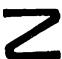
\includegraphics[keepaspectratio]{images/part002_676c5d74.jpg}}

注意，若 E 上的滤过是由 A 上的滤过导出的（例 2），则 E/F 上的商滤过也是，但 F 上诱导的滤过一般不是（习题 1；不过可参看 § 3 第 2 节定理 2）。

若 \(E'\) 是另一个滤过 A-模，则 \(E \times E'\) 上的乘积滤过与它的 A-模结构相容。若 E 与 \(E'\) 上的滤过都是由 A 上的滤过导出的（例 2），则它们的乘积滤过也是。
